\chapter{Applications}
\label{chap:applications}

\boitemagique{Objectif}{
Dans de ce chapitre nous présentons deux exemples d'applications de MDFT sur des systèmes biologiques. Le premier exemple permet d'évaluer la qualité de la prédiction de la structure de solvatation et le second permet dévaluer l'autre pan de MDFT soit la prédiction des énergies libres de solvatation.
}

Jusqu'ici, nous avons montré la façon dont nous avons étendue la théorie derrière MDFT et adapté le code afin de permettre l'étude de systèmes biologiques. Pour rappel, MDFT permet la prédiction (i) des structures du solvant et (ii) des énergies libres de solvatation de systèmes complexes. Dans ce chapitre, nous présentons deux exemples d'applications sur des systèmes biologiques, Le premier exemple permet d'évaluer la qualité de la prédiction de la structure de solvatation autour de macromolécules et le second permet dévaluer la prédiction des énergies libres de liaison et donc de solvatation de complexes protéines ligands.


\clearpage
\section{Application 1: Peut on retrouver les molécules d'eau cristallographiques?}
Certaines molécules d'eau jouent un rôle important dans la stabilité et le rôle des systèmes biologiques. Ces molécules interagissent entre elles ainsi qu'avec les systèmes biologiques via des liaisons hydrogènes. Comme il à été montré par Papoian et al. \cite{papoian_water_2004} l'eau joue un rôle dans le repliement et la liaisons des protéine via des interactions courtes portées mais également via des liaisons longues portées. Ces molécules sont donc indispensables à la bonne compréhension des différents processus biologiques ayant lieux dans le corps humain. Il existe différentes approches, expérimentales ou théoriques, permettant de détecter ces molécules.

Expérimentalement, ces molécules d'eau sont liées aux systèmes biologiques via un réseau de liaisons hydrogènes. Lors de la cristallisation d'une protéine par exemple, ces liaisons figent une partie des molécules de solvant, ce qui les rends alors détectables lors de la résolution expérimentale de la structure en 3 dimensions de tels systèmes. A cause des conditions nécessaires à la cristallisation \cite{wlodawer_advanced_2017} (agent précipitant, pH, température, ...), certaines liaisons vont être favorisées et d'autres vont être affaiblies. Les molécules d'eau expérimentalement détectées ne correspondent qu'en partie à celles que l'on retrouverait dans les conditions du laboratoire. Une fois publiées, ces structures sont, pour une majorité d'entre elles, ajoutées à la \textit{Protein Data Bank}\cite{pdb_2011} (PDB). La PDB est la base de données collaborative de référence pour les structures expérimentales de composés biologiques.

Il existe également différentes méthodes théoriques permettant la prédiction des molécules d'eau. Azuara et Al. proposent par exemple leur logiciel Aquasol \cite{azuara_pdb_hydro_2006} disponible en ligne et gratuit \footnote{\url{http://lorentz.dynstr.pasteur.fr/suny/index.php?id0=aquasol}}. Cette méthode implicite, basée sur la résolution de l'équation de Poisson Boltzmann permet de prédire une densité en eau autour d'une macromolécule. Il existe également des méthodes explicites comme celle proposée par Schrödinger à travers son logiciel WaterMap\cite{abel_role_2008}. Afin de prédire la position des molécules d'eau, une dynamique moléculaire de 10 ns est effectuée puis une carte de densité en eau est générée. Les molécules d'eau sont ensuite reconstruites en partant des maximums locaux de la densité. 


Cette étude à pour but d'évaluer la capacité de MDFT à retrouvée les molécules d'eau cristallographiques. En effet, comme nous l'avons décrit ci-dessus ces molécules sont intégrées à des réseaux de liaisons hydrogènes ce qui limite fortement leur mouvement. En d'autres termes, ces molécules peut être considérée comme fixes et par conséquent la probabilité de trouver une molécule d'eau à cet endroit est élevée. Ces molécules doivent donc se trouver dans des zones de fortes densité ou de forte probabilité de présence prédites par MDFT. Dans cette partie, nous comparons dans un premier temps, les résultats obtenus par MDFT et ceux obtenus par dynamique moléculaire, notre référence, sur des systèmes complexes. Dans un second temps nous vérifions l'adéquation entre les zones de forte probabilité de présence fournies par ces deux méthodes et la position des molécules d'eau expérimentales. Nous allions ainsi la rapidité des méthodes implicites comme Aquasol à la précision des méthodes explicites comme la dynamique moléculaire. 






\subsection{Les systèmes étudiés}
Afin de mener cette étude, la protéine \textit{Streptomyces Erythraeus Trypsin}, composée de 227 acides aminés, et issue de la PDB sous le code 4M7G, à été sélectionnée pour la qualité de sa résolution expérimentale (0.81 \AA).
%La seconde est une \textit{FACTOR XA} composée de 241 acides aminés. Cette protéine issue de la PDB [lien pdb] sous le code 1HCG à été sélectionnée car elle représente un premier cas d'étude simple, sans ligand ni contre ions.

%\begin{figure}[H]
%    \begin{subfigure}[b]{0.50\textwidth}
%        \centering
%        \resizebox{\linewidth}{!}{
%          \fbox{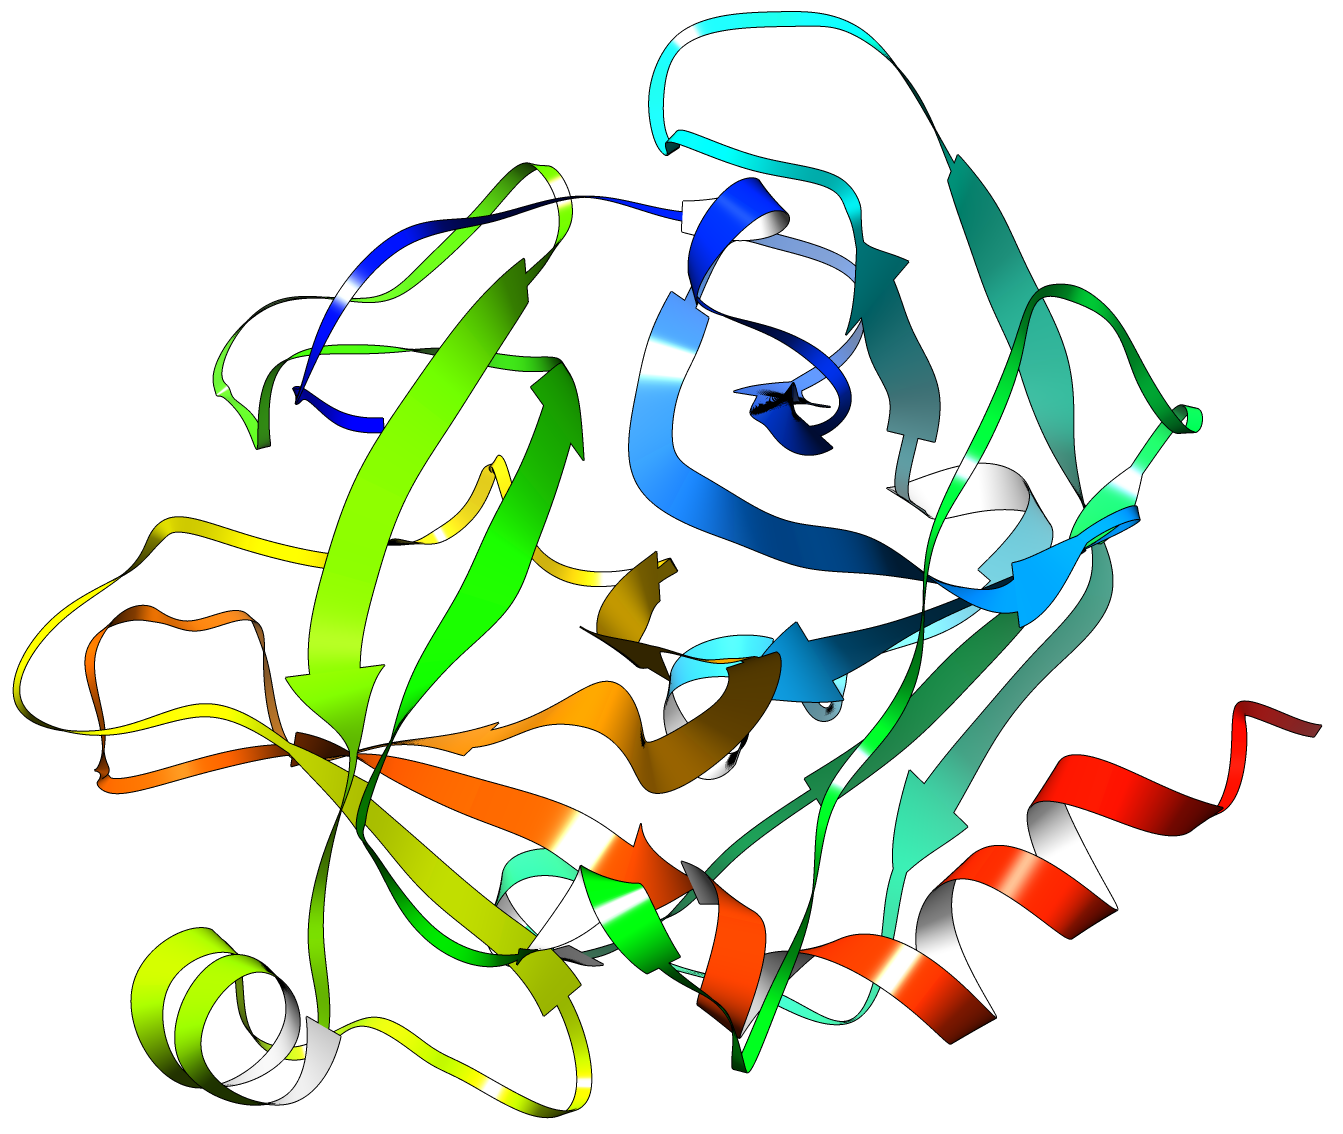
\includegraphics[width=\textwidth]{chapters/Applications/images/4m7g.png}}
%           }
%        \caption{4M7G}
%        \label{fig:struct_secondaire_4M7G}
%     \end{subfigure}
%    \begin{subfigure}[b]{0.50\textwidth}
%        \centering
%        \resizebox{\linewidth}{!}{
%	      \fbox{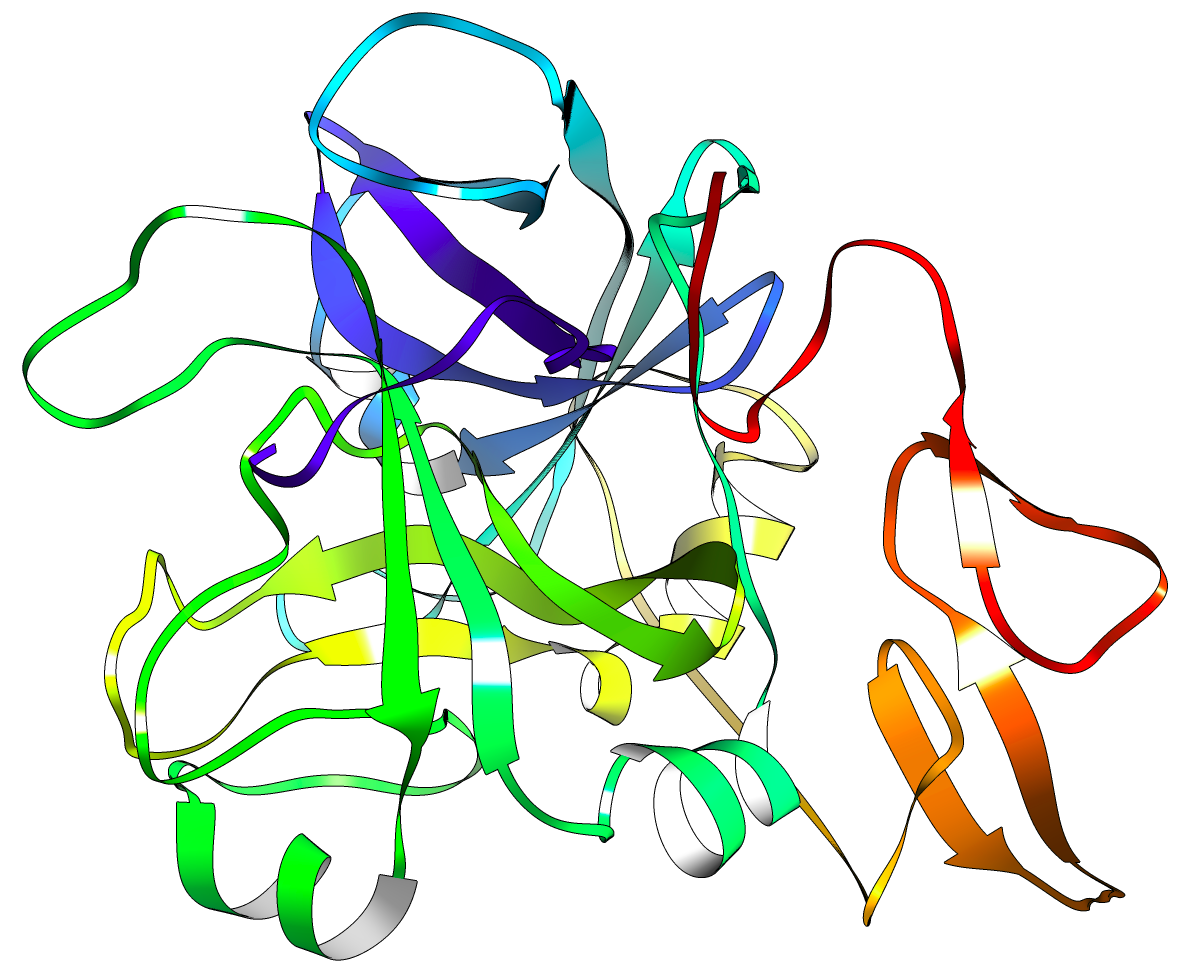
\includegraphics[width=\textwidth]{chapters/Applications/images/1hcg.png}}
%          }
%        \caption{1HCG}
%        \label{fig:struct_secondaire_1HCG}
%     \end{subfigure}
%   \caption{Représentation en structure secondaire des protéines 4M7G \ref{fig:struct_secondaire_4M7G} et 1HCG \ref{fig:struct_secondaire_4M7G}. }
%   \label{fig:struct_secondaires}
%\end{figure}

\begin{figure}[H]
   \centering
   \fbox{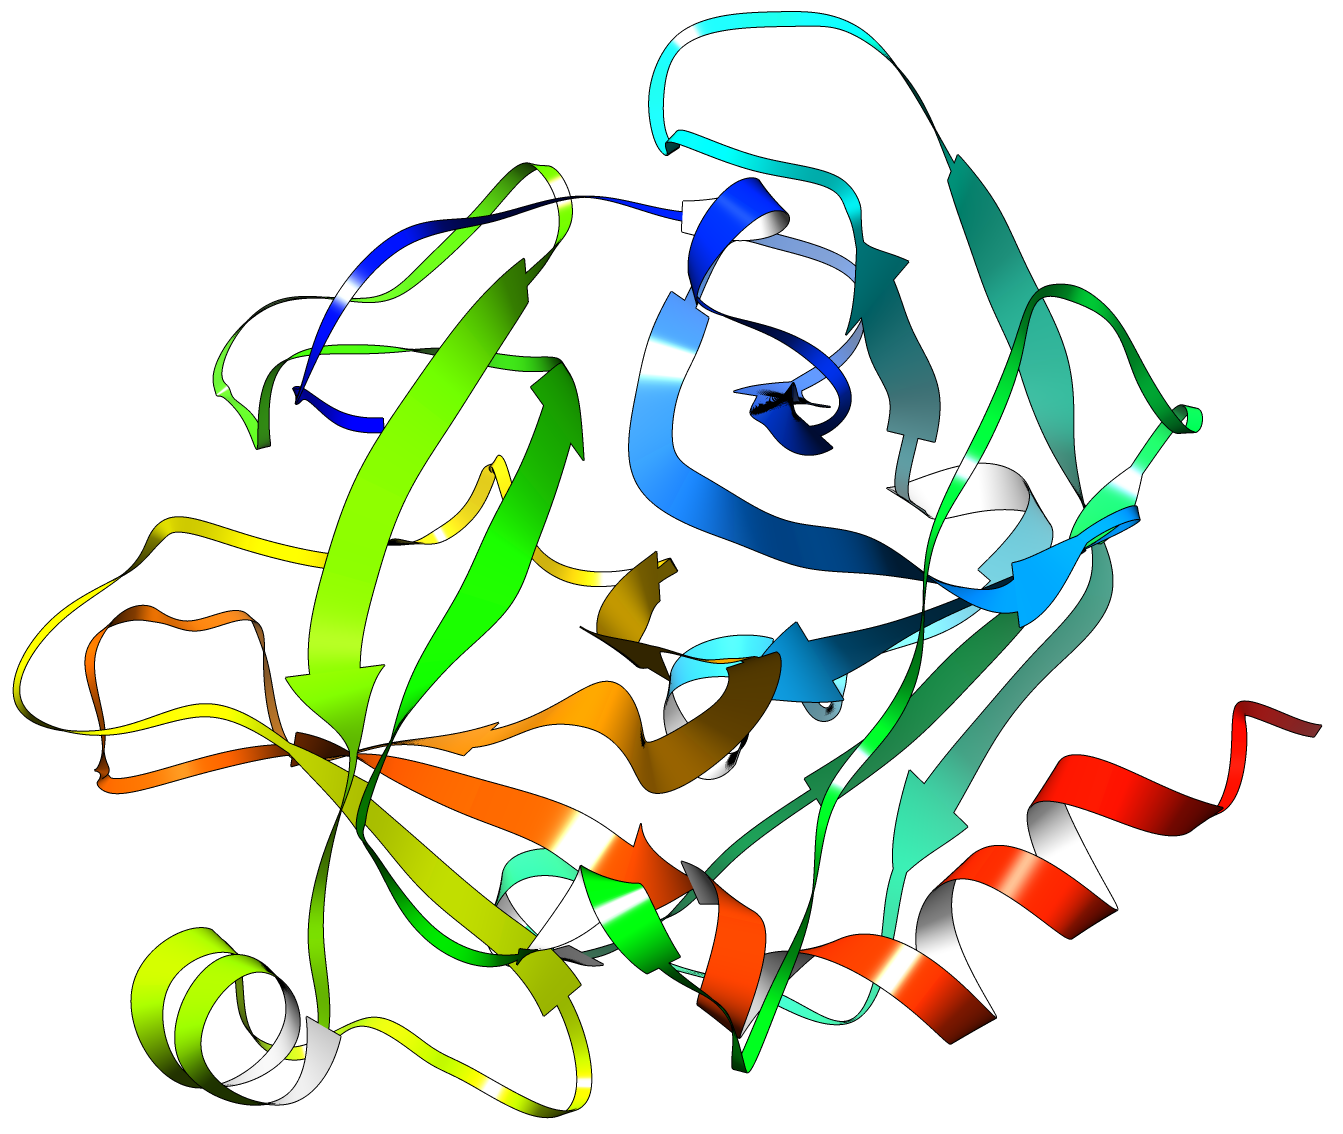
\includegraphics[width=\textwidth]{chapters/Applications/images/4m7g.png}}
   \caption{Représentation en structure secondaire de la protéine 4M7G. }
   \label{fig:struct_secondaires}
\end{figure}


\subsection{Protocole}

\subsubsection{Récupération et nettoyages de fichiers PDB}
Afin de ne pas être influencé par les résultats expérimentaux, nous avons suivi le protocole ( voir image \ref{fig:water_molecule_protocol}) suivant: Le structure 3D de notre molécule à été téléchargée depuis le site de la PDB [référence PDB] sous le code 4M7G. Ce fichier comporte la structure 3D de la protéine ainsi que d'éventuels ions ou molécules d'eau détectés expérimentalement. Les molécules d'eau ont été supprimées du fichier pdb afin de lancer les calculs MDFT et DM. Il n'y à donc à ce stade plus aucune trace de molécules d'eau expérimentales. Notre système est ensuite préparé en utilisant le champs de force OPLS/AA\cite{jorgensen_opls_1988} et le modèle d'eau SPC/E\cite{berendsen_missing_1987}. Pour chacune des méthodes (MDFT et DM), nous avons laissé un espace de 10 \AA\ entre les bords de notre boite de simulation et le bord de notre protéine. Chaque simulation à été effectué à 298.15 K.



\begin{figure}[H]
  \center
  \begin{tikzpicture}
  \tikzstyle{lien}=[->,>=stealth,rounded corners=5pt,thick]
  \node[inner sep=0pt] (protein_water) at (0,0)
      {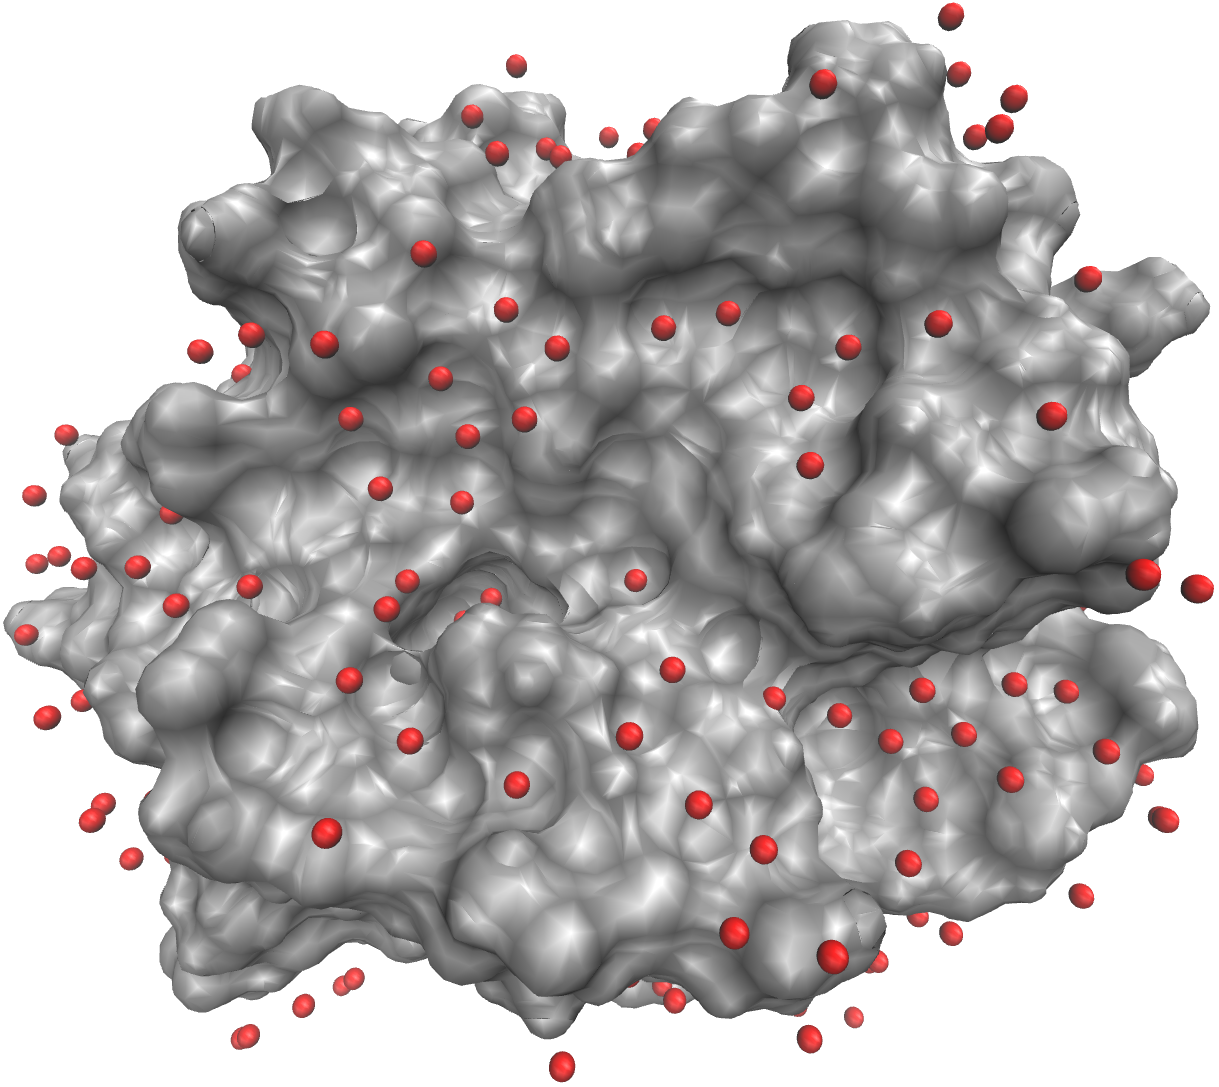
\includegraphics[width=.25\textwidth]{chapters/Applications/images/water_molecules_grey/prot_eau.png}};
  \node[inner sep=0pt] (water) at (6,0)
      {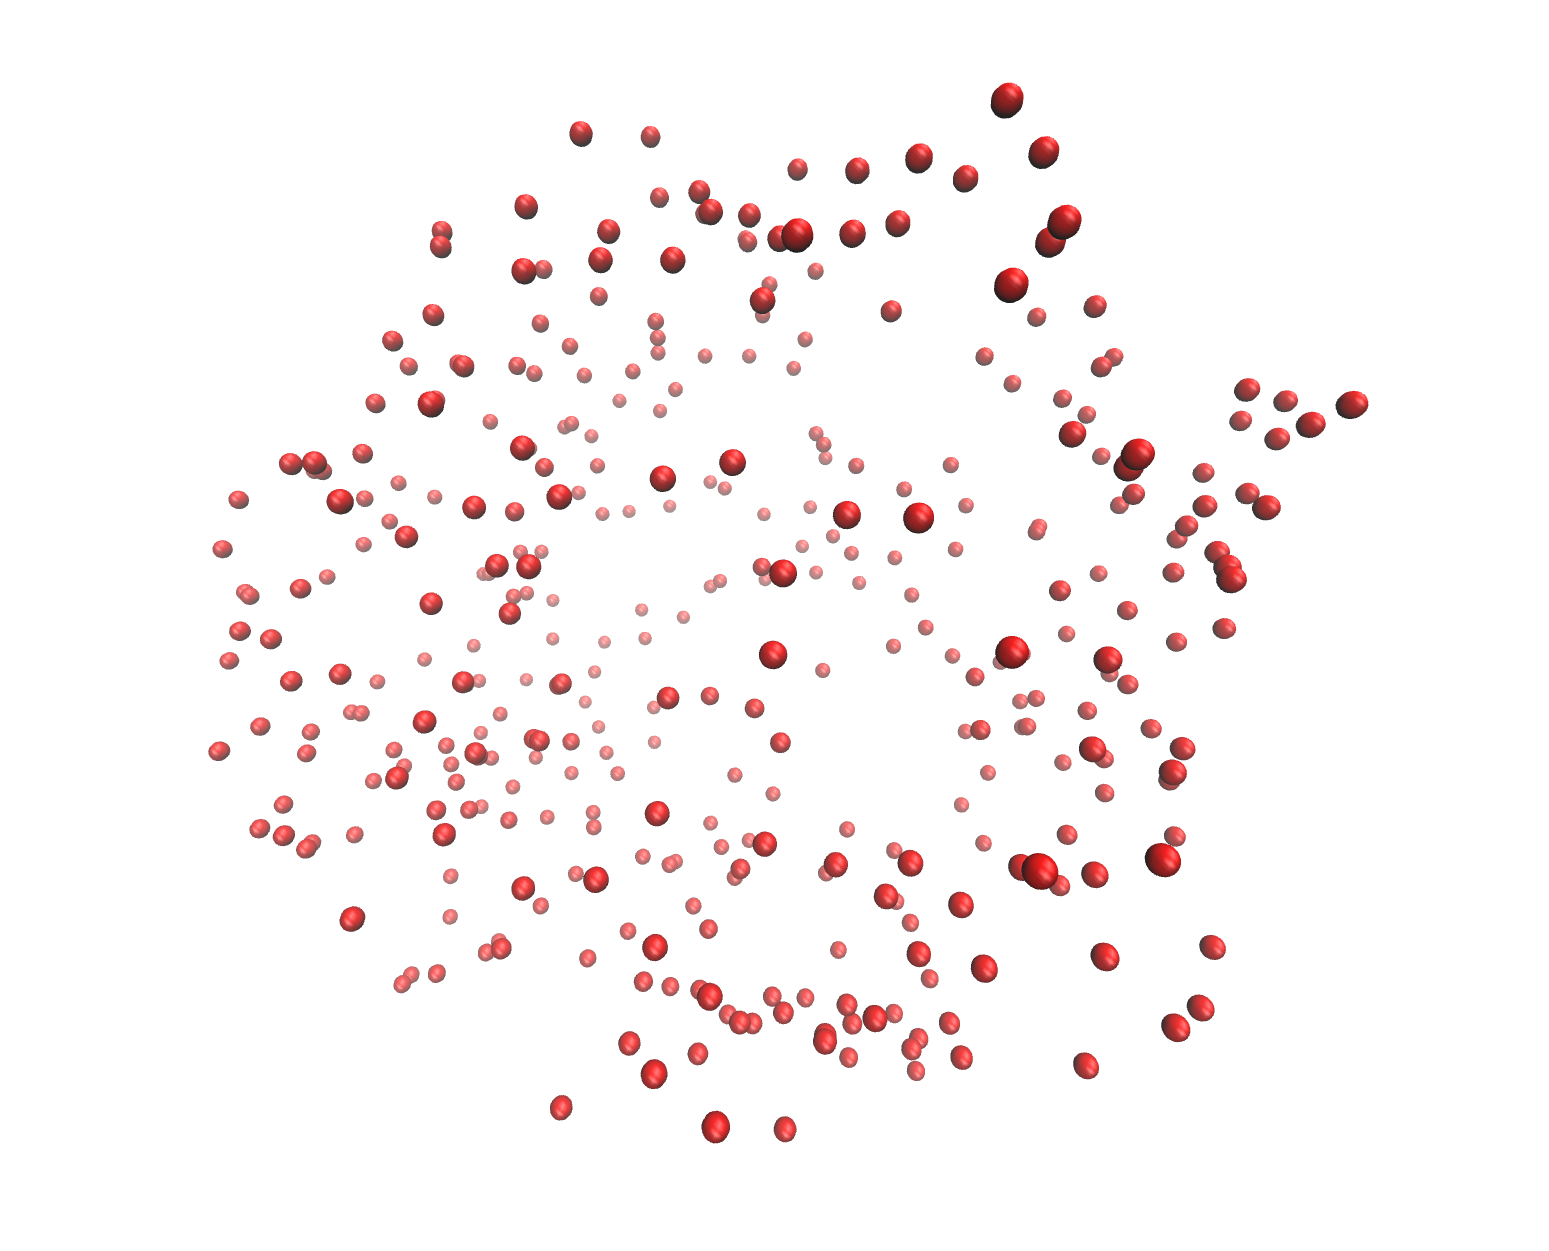
\includegraphics[width=.30\textwidth]{chapters/Applications/images/water_molecules/water.png}};
  \node[inner sep=0pt] (protein) at (12,0)
      {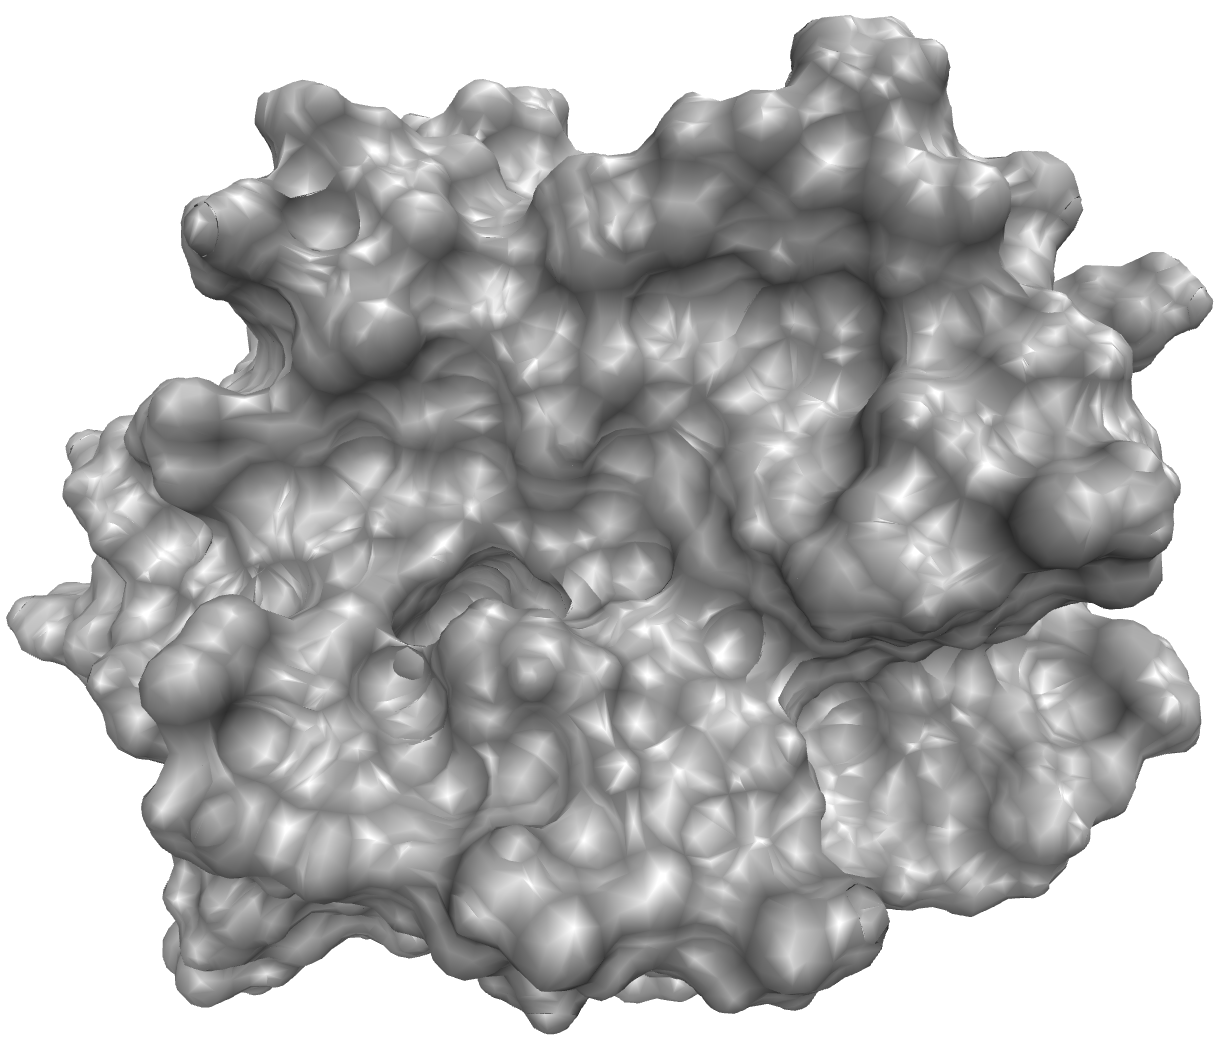
\includegraphics[width=.25\textwidth]{chapters/Applications/images/water_molecules_grey/prot.png}};
  \node[inner sep=0pt] (protein_water_2) at (0,-6)
      {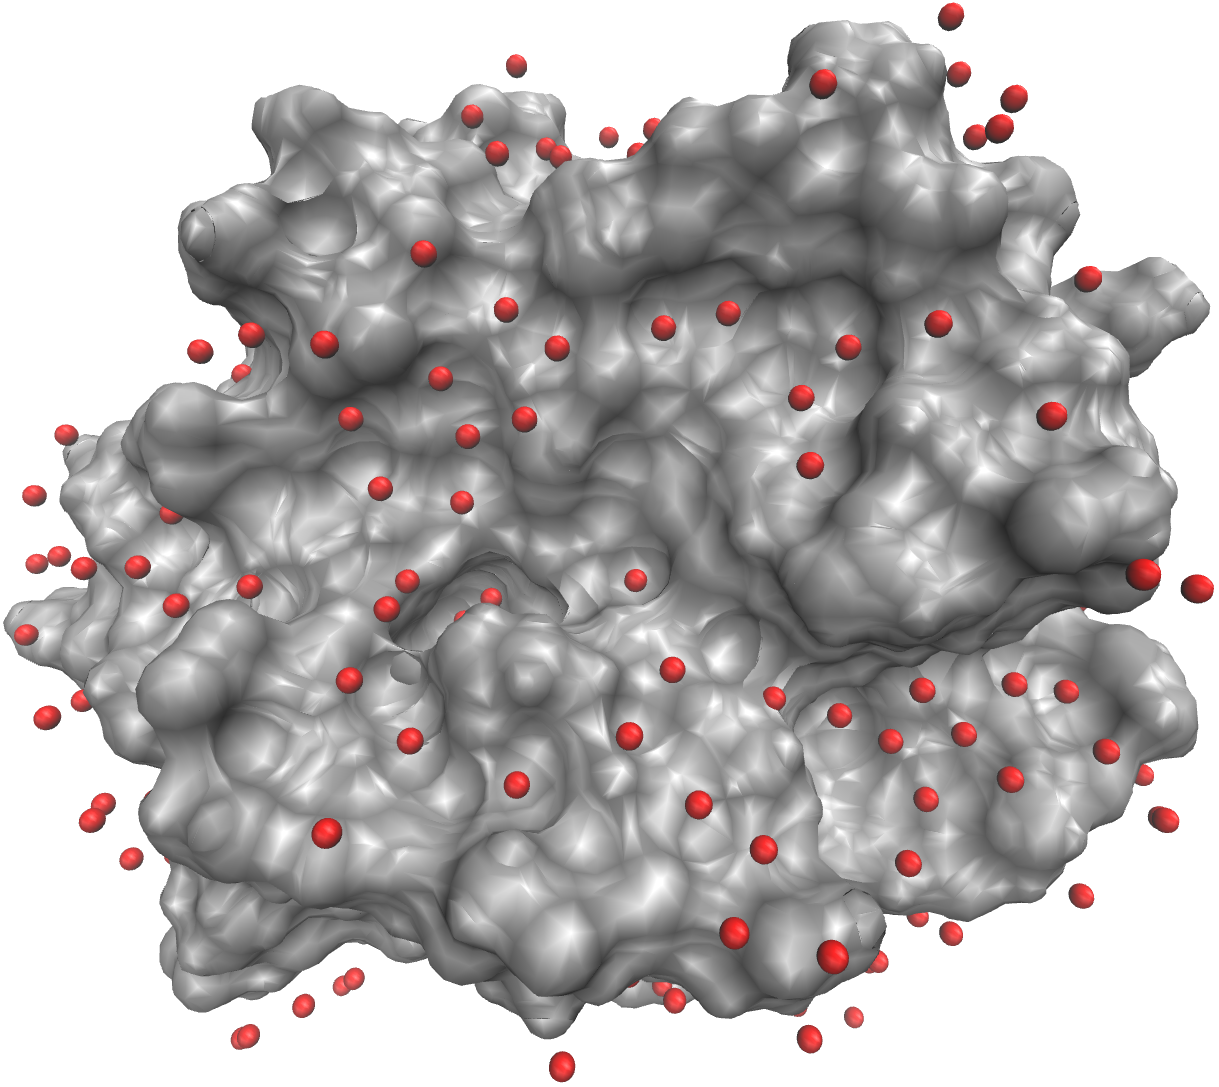
\includegraphics[width=.25\textwidth]{chapters/Applications/images/water_molecules_grey/prot_eau.png}};
  \node[inner sep=0pt] (protein_gromacs_water) at (6,-6)
      {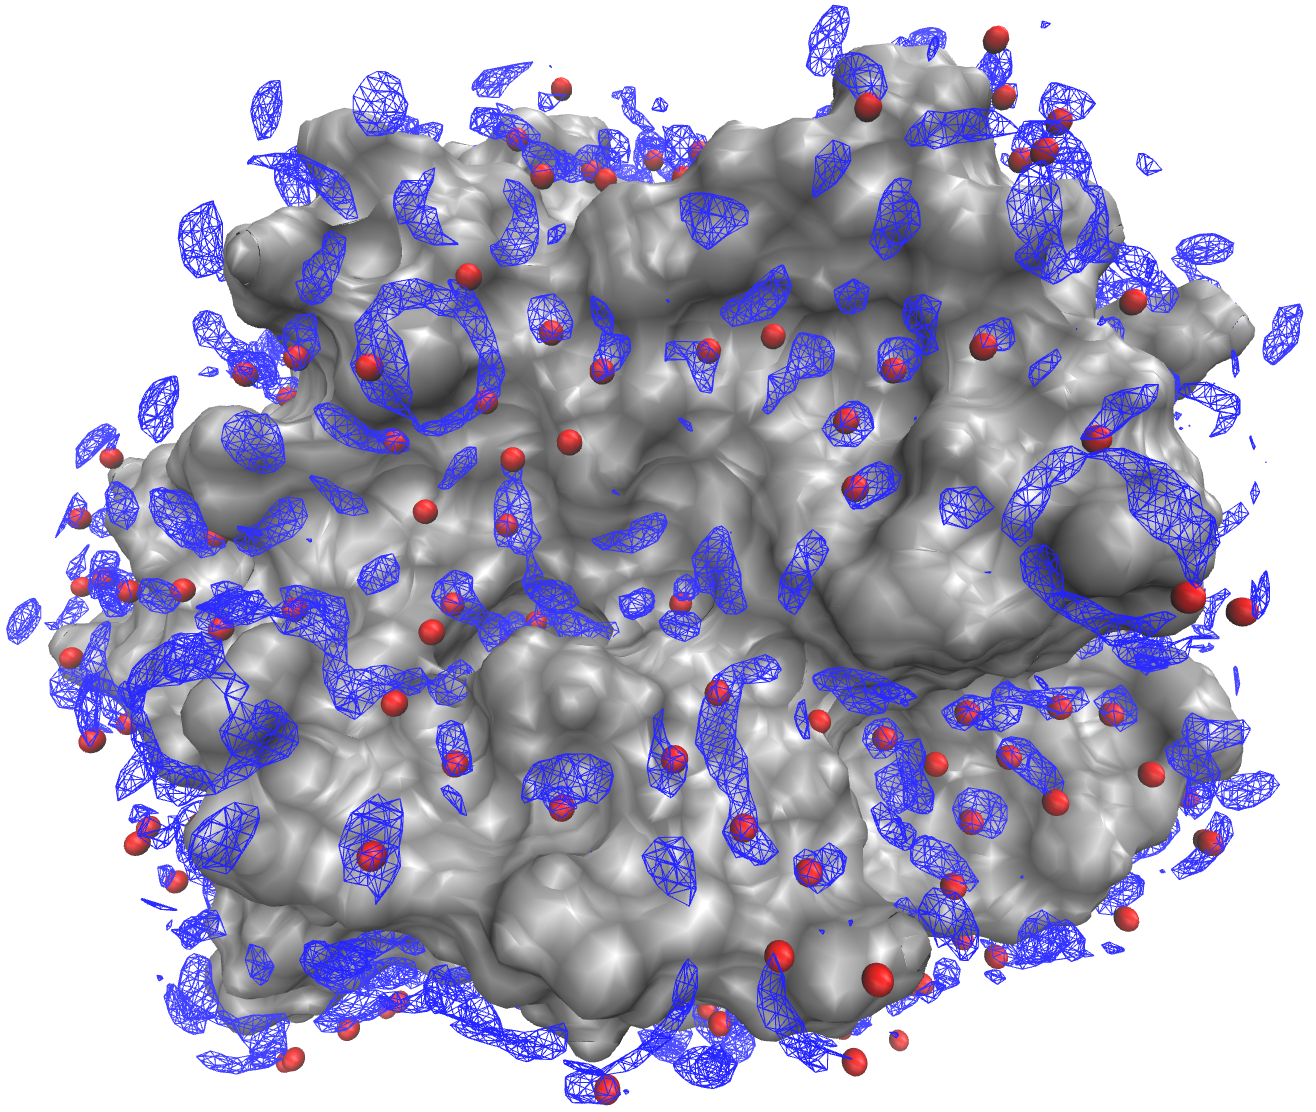
\includegraphics[width=.25\textwidth]{chapters/Applications/images/water_molecules_grey/prot_eau_md.png}};
  \node[inner sep=0pt] (protein_mdft_water) at (12,-6)
      {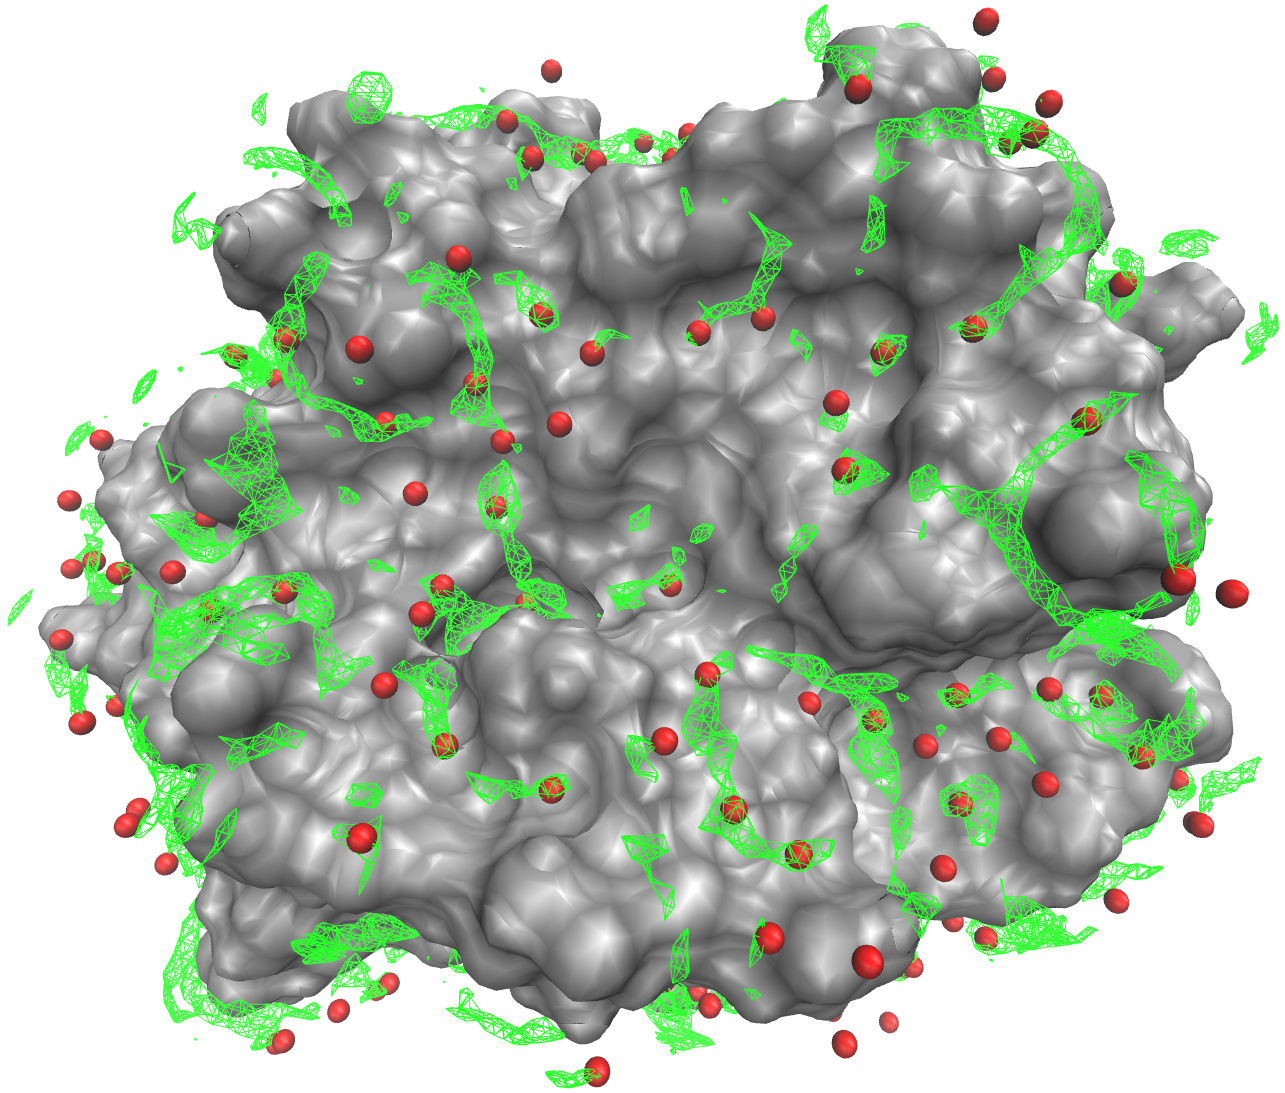
\includegraphics[width=.25\textwidth]{chapters/Applications/images/water_molecules_grey/prot_eau_mdft.png}};


  \draw[line width=5pt,red] (7.5, 1.5)--(4.5,-1.5);
  \draw[line width=5pt,red] (7.5,-1.5)--(4.5, 1.5);

  \draw (8.5,0) node[right] {+};


  \node[draw] (MDFT) at (12,-3) {MDFT};
  \node[draw] (MD) at (6,-3) {MD};

  \draw[-latex] (protein_water) -- (protein_water_2);
  \draw[-latex] (protein_water) -- (water);
  
  \draw[-latex] (protein.south) -- (MDFT.north);
  \draw[-latex] (protein.south) |- (6,-2 ) -- (MD.north);
  
  \draw[-latex] (MDFT.south) -- (protein_mdft_water.north);
  \draw[-latex] (MD.south) -- (protein_gromacs_water.north);
  
  \end{tikzpicture}
      \caption{Protocole de détection des molécules d'eau autour de la protéine 4M7G. La protéine est représentée en surface. Les sphères rouges correspondent aux molécules d'eau cristallographiques. Les zones de forte probabilité de présence proposées par dynamique moléculaire sont en bleu et celle proposées par MDFT sont en vert.}
      \label{fig:water_molecule_protocol}
\end{figure}




\subsubsection{Dynamique moléculaire}
Un calcul de référence à été lancé en dynamique moléculaire en utilisant le logiciel Gromacs\cite{berendsen_gromacs:_1995}. Après avoir solvaté nos protéines dans de l'eau SPC/E, l'énergie interne du système est minimisée, d'abord par steepest descent puis par gradient conjugué. Nous supprimons ainsi tous les clash stériques créés lors des étapes de préparation du système et de solvatation. Afin de permettre la comparaison des résultats avec ceux proposés par MDFT, la protéine est rendue rigide en utilisant l'option freezegrps proposée par gromacs. Lorsque cette option est activée, les forces appliquées aux atomes de la protéines sont ignorées. Le système est ensuite équilibré à 298.15K et 1 bar en utilisant le barostat Berendsen et le thermostat \textit{V-rescale}. Une fois le système proche de l'équilibre, nous changeons le barostat pour Parinello-Rahman qui est plus précis mais diverge si le système est trop éloigné de l'équilibre . Une fois le système minimisé, nous laçons une simulation NPT de 100 ns. La configuration du système est sauvegardée toutes les 10 ps, nous obtenons ainsi un ensemble 10 000 conformations. Sur 32 coeurs openMP/MPI, couplés à deux GPU, une simulation nécessite deux jours de calculs.

\subsubsection{MDFT}
Comme nous l'avons montré dans les chapitres précédents, avec notre bridge gros grain, $\mathrm{m}_\mathrm{max}$=3 est suffisant pour améliorer fortement la prédiction de structures de solvatation autour de petites molécules. Nous avons cependant choisi de lancer la simulation avec $\mathrm{m}_\mathrm{max}$=5 afin que cet exemple serve en même temps de test de robustesse de la nouvelle implémentation de MDFT. En effet, avec un espacement entre chaque point de grille de 0.5 \AA, MDFT minimise plus de $2\mathrm{e}^9$ de variables. Sur 16 cœurs openMP, les résultats sont obtenus en seulement 17 min.


\subsubsection{Conversion xtc en cube}
Pour comparer ces deux méthodes, nous avons développé un logiciel permettant de convertir une trajectoire XTC, fournie par gromacs, en une représentation statistique 3D au format CUBE. Ce logiciel, librement accessible sur github \footnote{\url{https://github.com/cgageat/xtc2Cube}} , découpe l'espace sous forme d'une grille ayant les même paramètres que celle utilisée par MDFT (ici 0.5 \AA\ de maille) puis, compte, pour chaque étape de la simulation, le nombre de molécules présentes dans chaque voxels. Ce total est ensuite divisé par le nombre d'étapes de simulation puis par la taille d'un voxel (voir équation \ref{eq:equationXtcToCube}). Nous obtenons ainsi une probabilité de présence en eau à l'équilibre pour chaque voxel, $\mathrm{n}\left(\boldsymbol{r}\right)$, qui est la même que celle obtenue à l'issue d'un calcul MDFT, c'est à dire le g($\boldsymbol{r}$). Cela nous permet ainsi une comparaison directe de ces deux méthodes.

\begin{equation}\label{eq:equationXtcToCube}
\mathrm{n}\left(\boldsymbol{r}\right) = \frac{1}{NV_{\boldsymbol{r}}}\sum\limits_{i=1}^N n(\boldsymbol{r}, i)
\end{equation}
 

\subsection{Résultats}
\subsubsection{En surface}
Dans un premier temps, nous évaluons l'efficacité de notre bridge en comparant les zones de forte probabilité de présence prédites en utilisant MDFT dans l'approximation HNC ( en jaune) puis avec notre bridge ( en vert ) à notre référence calculée par dynamique moléculaire ( en bleu ). Comme nous le voyons sur la figure \ref{fig:surface_protein_hnc}, l'approximation HNC surestime fortement la densité ou la probabilité de présence d'une molécule d'eau à de nombreux endroits. Notre bridge corrige cet effet et produit une carte de densité ayant une bien meilleure adéquation avec celle fournit par notre référence. Nous rappelons au lecteur que MDFT est 1 000 fois plus rapide que la dynamique moléculaire pour des calculs de structure de solvatation.







\begin{center}
    \captionsetup{type=figure}
	\fbox{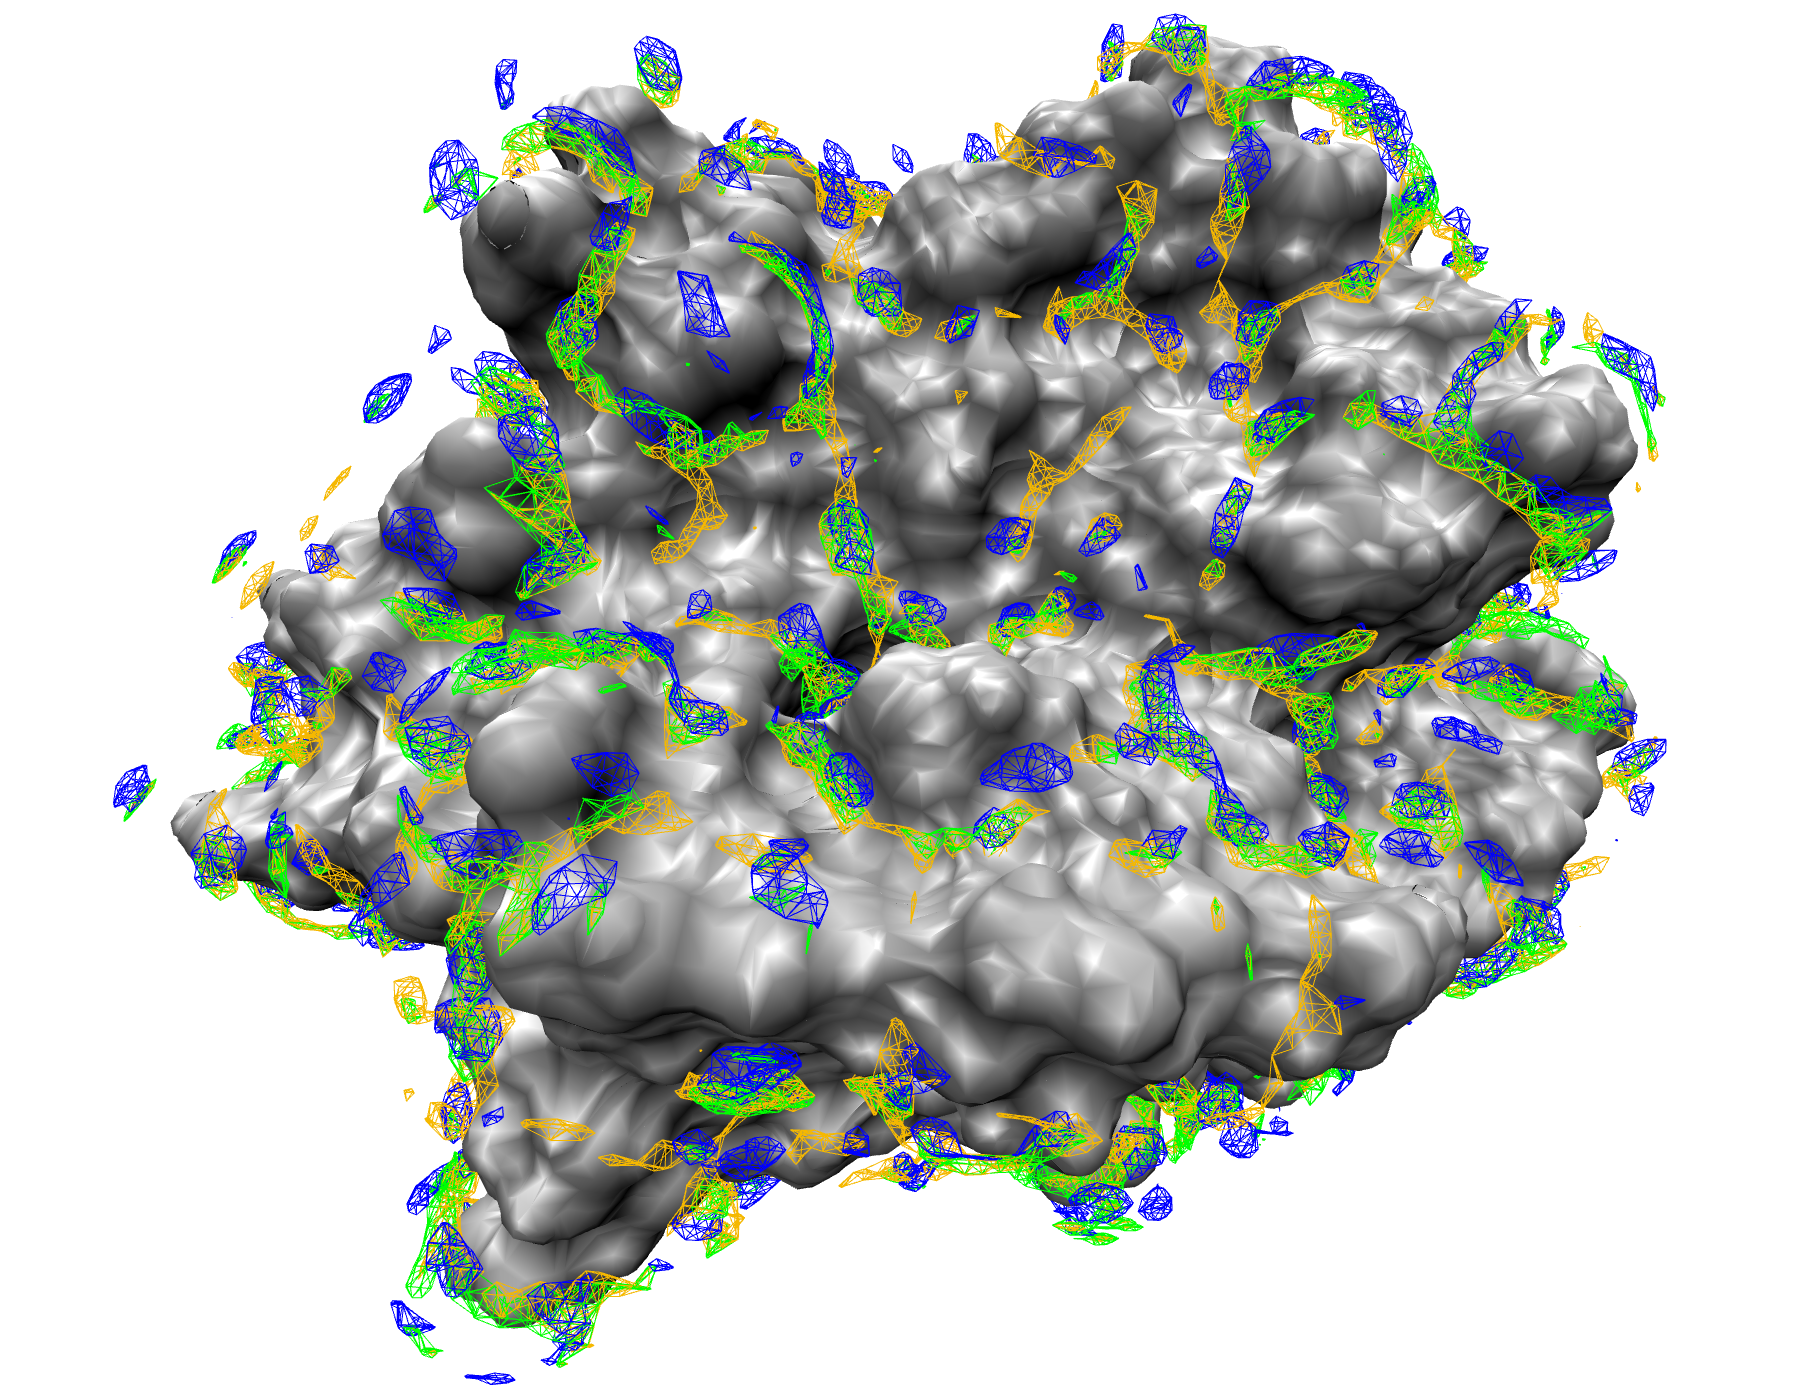
\includegraphics[width=\textwidth]{chapters/Applications/images/water_molecules_grey/prot_ext_hnc_bridge_md.png}}
	\captionof{figure}{ Zones de forte probabilité de présence de l'eau autour de la surface de la protéine 4M7G. En jaune, les zones prédites par MDFT dans l'approximation HNC et en vert MDFT avec notre nouveau bridge. La référence, en bleu, est calculée par dynamique moléculaire. }
      \label{fig:surface_protein_hnc}
\end{center}


Dans un second temps, nous comparons la position de ces zones de fortes probabilités de présence à la position des molécules d'eau expérimentales. On voit sur l'image \ref{fig:surface_water_molecule} que la majorité des molécules d'eau se situent dans les zones de fortes probabilités de présence proposées à la fois en dynamique moléculaire et par MDFT avec notre nouveau bridge. Cependant, certaines molécules ne sont retrouvées ni en dynamique moléculaire ni par MDFT. Cette différence peut venir des conditions expérimentales indispensables à la cristallisation et donc à la résolution de la structure 3D. En effet, les résolutions cristallographiques ne sont possibles qu'après une forte modification du système (agent de précipitation, pH, température) qui à pour effet de figer de nouvelles molécules d'eau mais également d'en libérer certaines autres. Il est donc attendu qu'il y ai une différence entre les résultats expérimentaux et théoriques.




\begin{center}
    \captionsetup{type=figure}
	\fbox{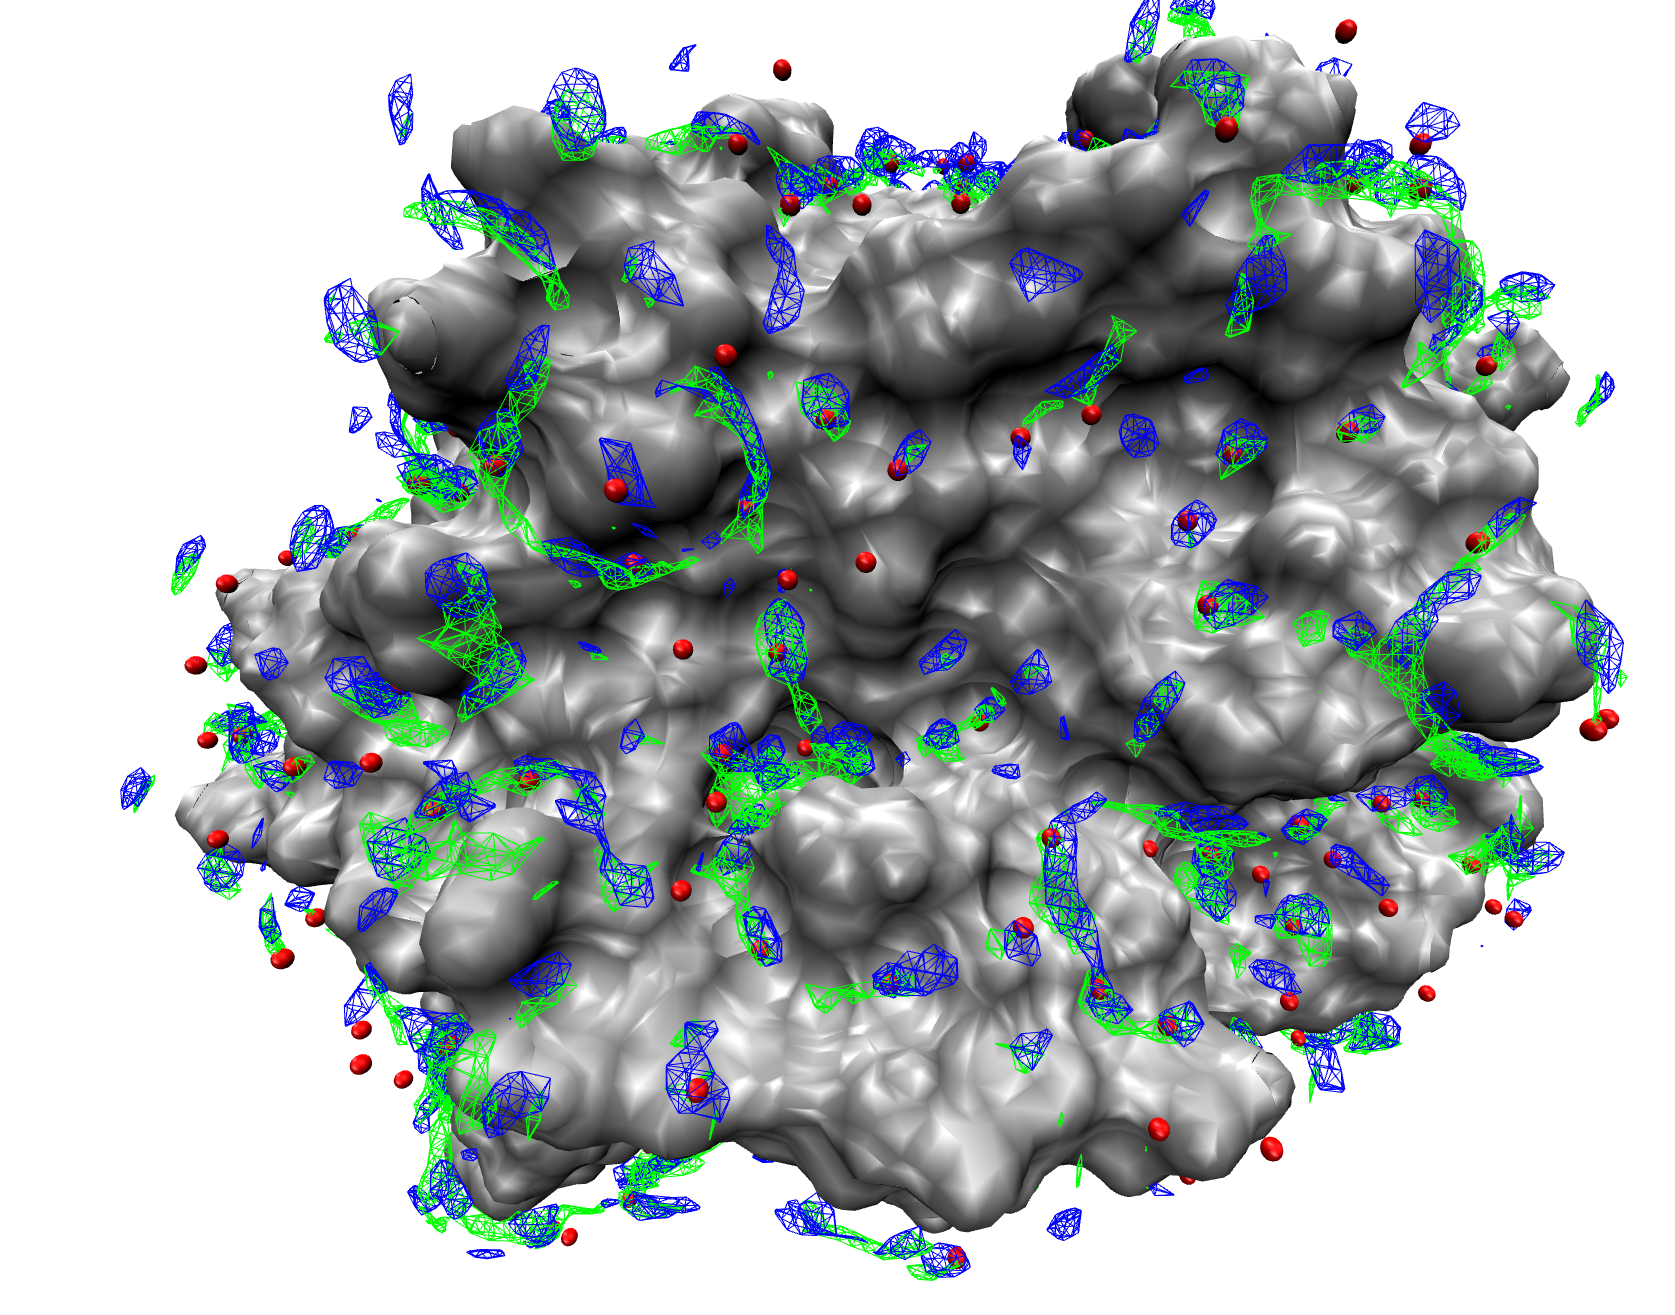
\includegraphics[width=\textwidth]{chapters/Applications/images/water_molecules_grey/prot_water_bridge_md}}
	\captionof{figure} {Comparaison des molécules d'eau cristallographiques et des résultats produits en dynamique moléculaire et par MDFT avec notre nouveau bridge à la surface de la protéine 4M7G. Les sphères rouges correspondent aux oxygènes des molécules d'eau cristallographiques. Les zones de forte probabilité de présence proposées par dynamique moléculaire sont représentées en bleu et celles proposées par MDFT sont en vert.}
      \label{fig:surface_water_molecule}
\end{center}



\subsubsection{A l'intérieur de la protéine}
La dernière partie de cette étude consiste à étudier notre solvant à l'intérieur des poches de la protéine. Comme on le voit sur la figure \ref{fig:interieur_water_molecule}, MDFT avec notre bridge (en vert) est en accord parfait avec les résultats expérimentaux. MDFT dans l'approximation HNC (en jaune) prédit de nombreuses zones de fortes densités qui ne correspondent à aucune molécule d'eau expérimentale comme c'est le cas en surface. De même, la dynamique moléculaire (en bleu) loupe deux molécules d'eau et en prédit plusieurs inexistantes. Ces résultats, pour la dynamique moléculaire, à l'intérieur de la protéine, s'expliquent par la dépendance des résultats de dynamique moléculaire aux conditions initiales. Durant les premières étapes d'une dynamique moléculaire le système est solvaté. A l'intérieur de la protéine, si une cavité est assez grande, des molécules d'eau y sont placées. En d'autre terme, si une cavité est anormalement grande dans cette configuration, une molécule y sera placée et restera bloquée tout au long de la simulation. A contrario, si une cavité est anormalement petite, aucune molécule d'eau n'y sera placée. Pour corriger cela, la protéine doit s'ouvrir durant la simulation, libérer ou absorber une molécule d'eau, puis se refermer. Ces phénomènes, de l'ordre de la seconde, ne sont pas accessibles en dynamique moléculaire. MDFT propose des résultats directement à l'équilibre et permet donc une meilleure prédiction à l'intérieur des systèmes biologiques.




\begin{center}
    \captionsetup{type=figure}
	\fbox{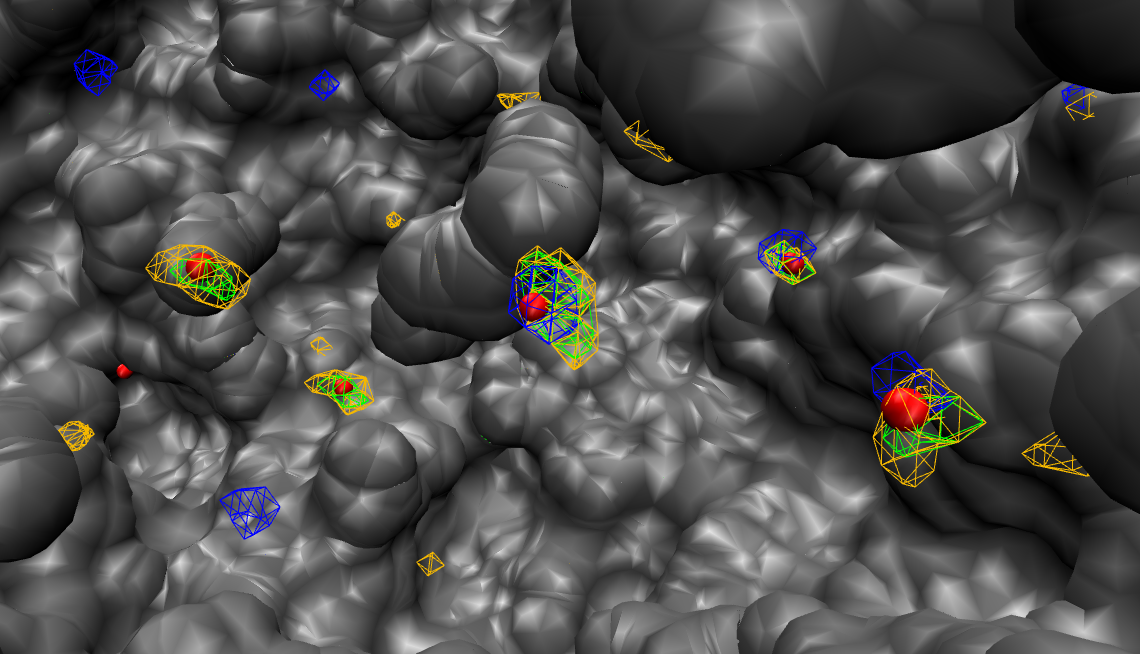
\includegraphics[width=\textwidth]{chapters/Applications/images/water_molecules_grey/prot_interieur_gris}}
	\captionof{figure}{Comparaison des molécules d'eau cristallographiques et des résultats produits en dynamique moléculaire et par MDFT à l'intérieur de 4M7G. La protéine est représentée en surface. Les sphères rouges correspondent aux molécules d'eau cristallographiques. Les zones de forte probabilité de présence proposées par dynamique moléculaire sont en bleu et celle proposées par MDFT sont en vert.}
      \label{fig:interieur_water_molecule}
\end{center}




\clearpage
\section{application 2: MM-MDFT pour remplacer MM-PBSA}
Lors du développement d'un nouveau médicament, les calculs d'énergies libres de liaison sont indispensables et interviennent à différentes étapes du procédé. Ils permettent par exemple d'évaluer l'affinité d'un petit composé, candidat médicament, avec (i) sa cible thérapeutique et ainsi d'évaluer son efficacité et (ii) avec des cibles secondaires et ainsi d'évaluer le risque d'effets secondaires. Durant les premières étapes, un premier tri large est effectué et la rapidité est favorisée à la précision. La méthode de choix est donc MM-PBSA\cite{genheden_mm/pbsa_2015}. Cette méthode implicite permet une évaluation quasi-instantanée de l'énergie libre de liaison en échange de fortes approximations. Un solvant implicite ne permet par exemple pas de prendre en compte les effets stériques des molécules d'eau ou encore les liaisons hydrogènes qu'elles pourraient former avec le complexe solvaté. Dans cette partie, nous dérivons MM-PBSA en une nouvelle méthode MM-MDFT. Les résultats MM-PBSA de 46 complexes protéine-ligand, récemment publiés par Cheron et Al.\cite{cheron_effect_2017}, sont comparés à ceux obtenus par MM-MDFT.

\subsection{Théorie}
Par définition, le calcul exact d'une énergie libre de liaison, implique un échantillonnage complet du système étudié. Dans le cas d'un complexe rigide protéine-ligand, ce calcul implique l'échantillonnage de toutes les conformations du solvant. Afin de simplifier et d’accélérer les calculs, il est d'usage d'appliquer le cycle thermodynamique (voir figure \ref{fig:Energie_libre_de_binding} ) suivant: Dans un premier temps, la protéine et le ligand sont désolvatés. Une fois dans le vide, le calcul de l'énergie libre de liaison correspond à la somme des termes inter et intra-moléculaires moyennés sur l'ensemble des conformations possibles. Dans le cas de molécules rigides, les énergies internes des deux composés ne sont pas modifiées lors de la liaison et peuvent donc être ignorées. L'énergie libre de liaison correspond ainsi à la somme des termes intra-moléculaires. Enfin, le complexe nouvellement formé est de nouveau solvaté. Comme nous l'avons détaillé dans le chapitre ( voir chapitre \ref{chap:introduction} ), il existe différentes méthode permettant le calcul de l'énergie libre de solvatation. Les systèmes biologiques ne permettent pas, de par leur taille, d'utiliser des méthodes explicites telles que l'intégration thermodynamique associées à des simulations de dynamique moléculaire ou de Monte Carlo. Les méthodes implicites telles que \textit{Poisson-Boltzman and Surface-Area} (PBSA) sont donc favorisées.



\begin{figure}[H]
  \center
  \begin{tikzpicture}
  
   \draw (0,0,0)--(3,0,0)--(3,3,0)--(0,3,0)--cycle;
   \draw (4,0,0)--(7,0,0)--(7,3,0)--(4,3,0)--cycle;
   \draw (11,0,0)--(14,0,0)--(14,3,0)--(11,3,0)--cycle;
   \draw[fill=white!70!cyan] (0,6,0)--(3,6,0)--(3,9,0)--(0,9,0)--cycle;
   \draw[fill=white!70!cyan] (4,6,0)--(7,6,0)--(7,9,0)--(4,9,0)--cycle;
   \draw[fill=white!70!cyan] (11,6,0)--(14,6,0)--(14,9,0)--(11,9,0)--cycle;

   \draw[fill=black] (5.4, 1.5) circle (1);
   \draw[fill=black] (12.4,1.5) circle (1);
   \draw[fill=black] (5.4, 7.5) circle (1);
   \draw[fill=black] (12.4,7.5) circle (1);
   \draw[gray,fill=gray] (2.1, 1.5) circle (0.5);
   \draw[white,fill=white] (6.1, 1.5) circle (0.5);
   \draw[gray,fill=gray] (13.1,1.5) circle (0.5);
   \draw[gray,fill=gray] (2.1, 7.5) circle (0.5);
   \draw[white!70!cyan,fill=white!70!cyan] (6.1, 7.5) circle (0.5);
   \draw[gray,fill=gray] (13.1,7.5) circle (0.5);

   \draw[line width=5pt, -latex] (7.5, 1.5) -- (10.5,1.5);
   \draw (8.8,1.4) node[below]{$\Delta G_{\mathrm{liaison}}\ \mathrm{vide}$} ;
   \draw[line width=5pt, -latex] (7.5, 7.5) -- (10.5,7.5);
   \draw (8.8,7.4) node[below]{$\Delta G_{\mathrm{liaison}}\ \mathrm{eau}$} ;

   \draw[line width=5pt, -latex] (1.5, 3.5) -- (1.5,5.5);
   \draw (1.5,4.3) node[right]{$\Delta G_{\mathrm{solv}}\ \mathrm{ligand}$} ;
   \draw[line width=5pt, -latex] (5.5, 3.5) -- (5.5,5.5);
   \draw (5.5,4.3) node[right]{$\Delta G_{\mathrm{solv}}\ \mathrm{protéine}$} ;
   \draw[line width=5pt, -latex] (12.5, 3.5) -- (12.5,5.5);
   \draw (12.5,4.3) node[right]{$\Delta G_{\mathrm{solv}}\ \mathrm{complexe}$} ;

  \end{tikzpicture}
    \caption{Cycle thermodynamique utilisé dans le calcul de l'énergie libre de liaison entre une protéine et un ligand par MM-PBSA et MM-MDFT.}
    \label{fig:Energie_libre_de_binding}
\end{figure}





\subsubsection{MM-PBSA}
MM-PBSA est une méthode, basé sur le cycle thermodynamique décrit ci-dessus, qui permet d'estimer, en quelques seconde seulement, l'énergie libre de liaison entre deux molécules dans un solvant implicite. Les énergies libres de solvatation sont calculées par PBSA et l'énergie libre de liaison est calculée par \textit{Molecular Mechanics}. PBSA est basée sur la résolution de l'équation de Poisson-Boltzmann (PB) pour les charges et sur le calcul de la surface accessible au solvant (SA). L’énergie libre de solvatation correspond à la somme de ces deux termes. 





\subsubsection{MM-MDFT}
MDFT calcule les énergies libres de solvatation, ce qui nous permet de remplacer les calculs PBSA par des calculs MDFT et ainsi de décliner MM-PBSA en MM-MDFT. Afin de rester comparable, nous avons fait le choix d'une approximation de la théorie MDFT, qui nous propose des résultats dans des temps équivalents à ceux fournis par PBSA, soit de l'ordre de la seconde. Nous avons donc fixé $\mathrm{m}_\mathrm{max}=1$, et testés les corrections de pression PC et PC+ ainsi que le bridge gros grain. Notre objectif ici n'est pas d'être plus rapide que MM-PBSA mais d'ajouter de la précision aux résultat tout en apportant des informations supplémentaires au travers de la structure de solvatation. 


\subsection{Les systèmes étudiés}
Dans une étude récente, Cheron et Al.\cite{cheron_effect_2017} ont optimisés le calculs MM-PBSA sur un ensemble de 46 complexes protéine-ligand. Afin de créer cette chimiothèque, l'ensemble des 264 complexes impliquant la protéine BACE1 ( voir figure \ref{fig:structure_proteine_MMPBSA} ) ont été extraits de la base de données PDBBind-CN. Parmi ces 264, seul 46 étaient de qualité suffisante (résolution < 2.5 \AA) et accompagnés de leur valeur d'énergie libre de solvatation. Dans leur article, Cheron et Al. montrent que les calculs MM-PBSA sur ces complexes sont optimums en utilisant le champs de force Amber03 pour la protéine, le modèle d'eau TIP3P et en laissant un espace supérieur à 10 \AA\ entre les molécules le composant et le bord des boites de simulation. Les valeurs d'énergies libre de solvatation expérimentales et calculées par MM-PBSA présentées dans la suite de ce chapitre ont toutes été fournies par Nicolas Cheron, actuellement en post-doctorat avec Damien Laage.

Le code PDB ainsi que les charges des différents complexes sont listés dans le tableau \ref{tab:MMPBSA_systemes}. Une représentation 2D des ligands de chaque complexe est également disponible en figure \ref{fig:structures_MMPBSA}.








\begin{center}
\begin{longtable}{ c c c c c }

%{{\bfseries \tablename\ \thetable{} -- première page}} \\
\hline
Code &  \multicolumn{3}{c}{Charge} & $\mathrm{N}_\mathrm{atomes}$ \\
PDB  & complex & protein & ligand  & Ligand \\ \hline 
\endfirsthead

\multicolumn{5}{c}%
{{\bfseries \tablename\ \thetable{} -- suite}} \\
\hline Code PDB &  \multicolumn{3}{c}{Charge} & $\mathrm{N}_\mathrm{atomes} \mathrm{Ligand}$ \\
               & complex & protein & ligand  & \\ \hline 
\endhead

\hline \multicolumn{5}{ r }{{Suite page suivante}} \\ \hline
\endfoot

\hline \hline
\caption{Description des systèmes utilisés dans l'étude MM-MDFT. Pour chaque système la charge du complexe, de la protéine et du ligand seuls sont indiqués ainsi que le nombre d'atome composant le ligand.} \label{tab:MMPBSA_systemes} \\
\endlastfoot

      \hline & \\[-1em]\hline
      
      \hline
      1FKN & -10.0 &  -8.0 & -2.0 & 125 \\
      1M4H & -11.0 &  -8.0 & -3.0 & 132 \\
      2FDP &  -9.0 & -10.0 &  1.0 &  83 \\
      2G94 & -10.0 & -10.0 &  0.0 &  99 \\
      2P4J & -10.0 & -10.0 &  0.0 & 104 \\
      2Q11 & -10.0 & -10.0 &  0.0 &  61 \\
      2Q15 &  -9.0 & -10.0 &  1.0 &  78 \\
      2QMG &  -9.0 & -10.0 &  1.0 &  84 \\
      3BRA &  -9.0 & -10.0 &  1.0 &  22 \\
      3BUF &  -9.0 & -10.0 &  1.0 &  25 \\
      3BUG & -10.0 & -11.0 &  1.0 &  28 \\
      3BUH &  -9.0 & -10.0 &  1.0 &  38 \\
      3CKP &  -9.0 & -10.0 &  1.0 &  80 \\
      3I25 & -10.0 & -10.0 &  0.0 & 118 \\
      3KMX &  -9.0 &  -9.0 &  0.0 &  34 \\
      3KMY &  -9.0 &  -9.0 &  0.0 &  29 \\
      3L59 & -14.0 & -14.0 &  0.0 &  31 \\
      3L5B & -10.0 & -10.0 &  0.0 &  40 \\
      3LPI &  -9.0 & -10.0 &  1.0 &  89 \\
      3LPK &  -9.0 & -10.0 &  1.0 &  91 \\
      3RSX & -10.0 & -10.0 &  0.0 &  26 \\
      3RU1 & -10.0 & -10.0 &  0.0 &  48 \\
      3UDH & -10.0 & -11.0 &  1.0 &  27 \\
      3WB4 & -10.0 & -10.0 &  0.0 &  37 \\
      3WB5 & -10.0 & -10.0 &  0.0 &  38 \\
      4B05 &  -9.0 &  -9.0 &  0.0 &  48 \\
      4DJU & -10.0 & -10.0 &  0.0 &  35 \\
      4DJV & -10.0 & -10.0 &  0.0 &  49 \\
      4DJW & -10.0 & -10.0 &  0.0 &  44 \\
      4DJX & -10.0 & -10.0 &  0.0 &  41 \\
      4DJY & -10.0 & -10.0 &  0.0 &  46 \\
      4FRS &  -9.0 &  -9.0 &  0.0 &  42 \\
      4FS4 & -10.0 & -10.0 &  0.0 &  45 \\
      4FSL & -10.0 & -10.0 &  0.0 &  57 \\
      4GID &  -9.0 & -10.0 &  1.0 &  95 \\
      4H1E &  -9.0 &  -9.0 &  0.0 &  54 \\
      4H3F & -10.0 & -10.0 &  0.0 &  55 \\
      4H3G & -10.0 & -10.0 &  0.0 &  52 \\
      4H3I & -10.0 & -10.0 &  0.0 &  55 \\
      4H3J & -10.0 & -10.0 &  0.0 &  52 \\
      4HA5 & -10.0 & -10.0 &  0.0 &  39 \\
      4R8Y &  -9.0 &  -9.0 &  0.0 &  70 \\
      4R91 &  -9.0 & -10.0 &  1.0 &  72 \\
      4R92 &  -9.0 &  -9.0 &  0.0 &  69 \\
      4R93 & -10.0 & -10.0 &  0.0 &  72 \\
      4R95 & -10.0 & -10.0 &  0.0 &  73 \\
\end{longtable}
\end{center}








\begin{center}
    \captionsetup{type=figure}
	\fbox{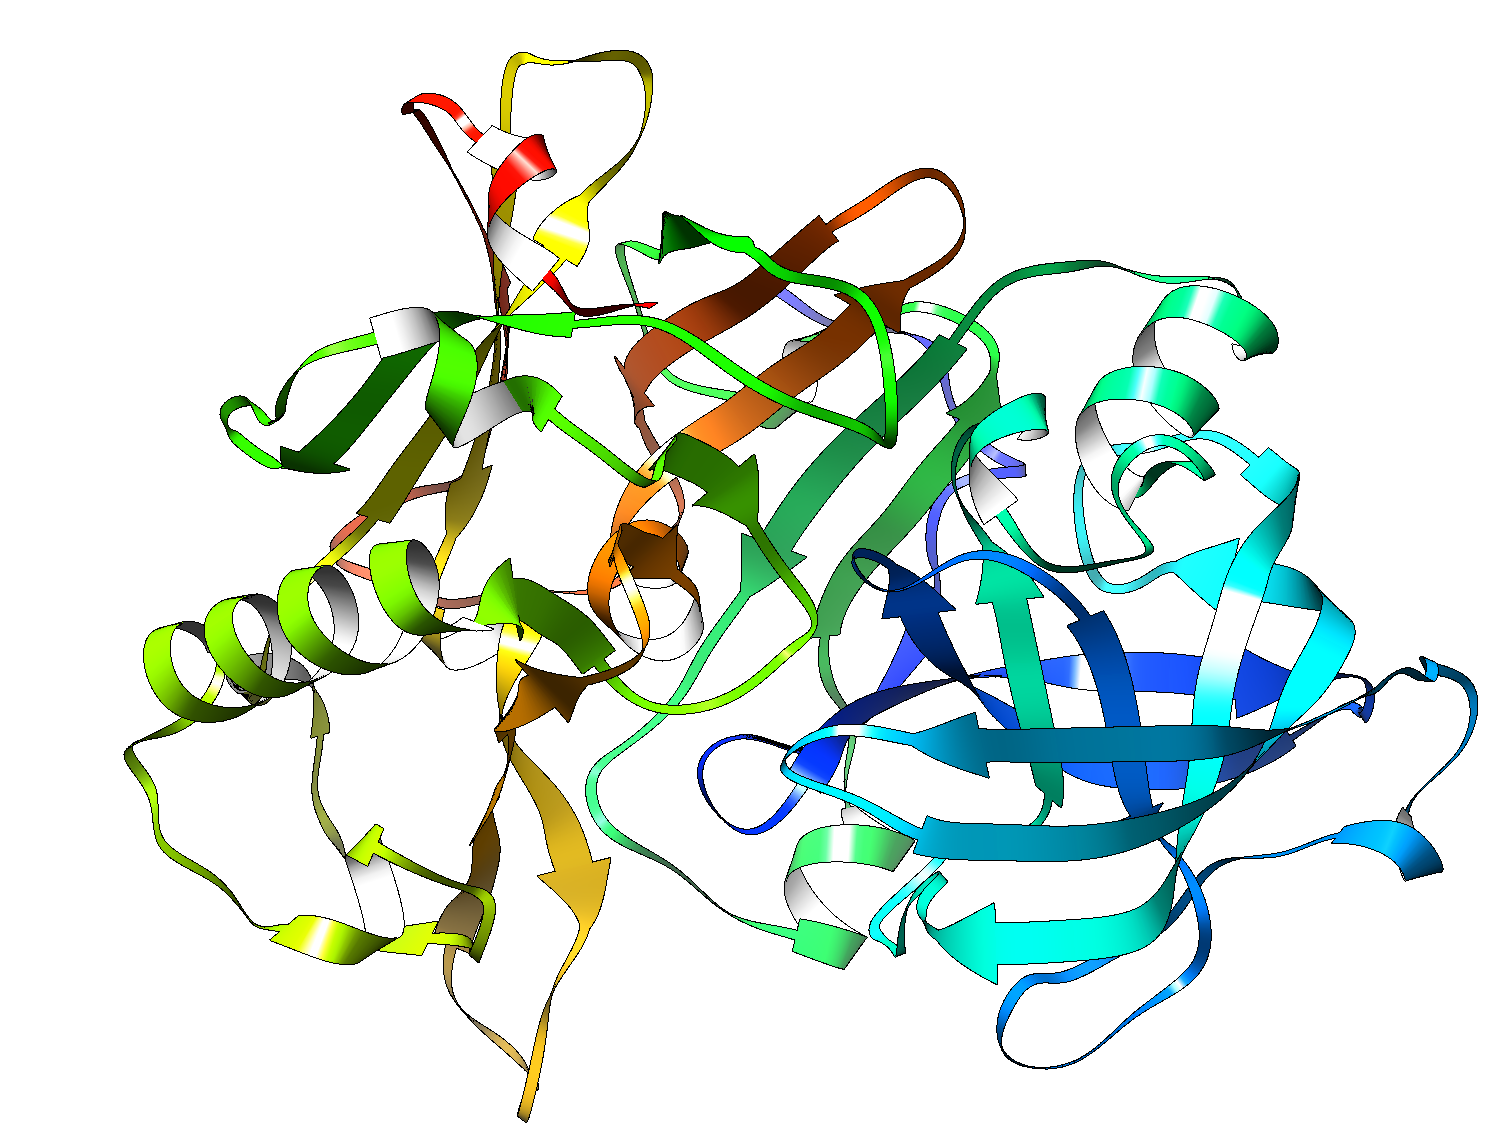
\includegraphics[width=0.8\textwidth]{chapters/Applications/images/structure_proteine_mmpbsa.png}}
	\captionof{figure}{Structure 3D de la protéine BACE1 en commun dans tous les complexes étudiés.}
    \label{fig:structure_proteine_MMPBSA}
\end{center}


\begin{center}
    \captionsetup{type=figure}
	\fbox{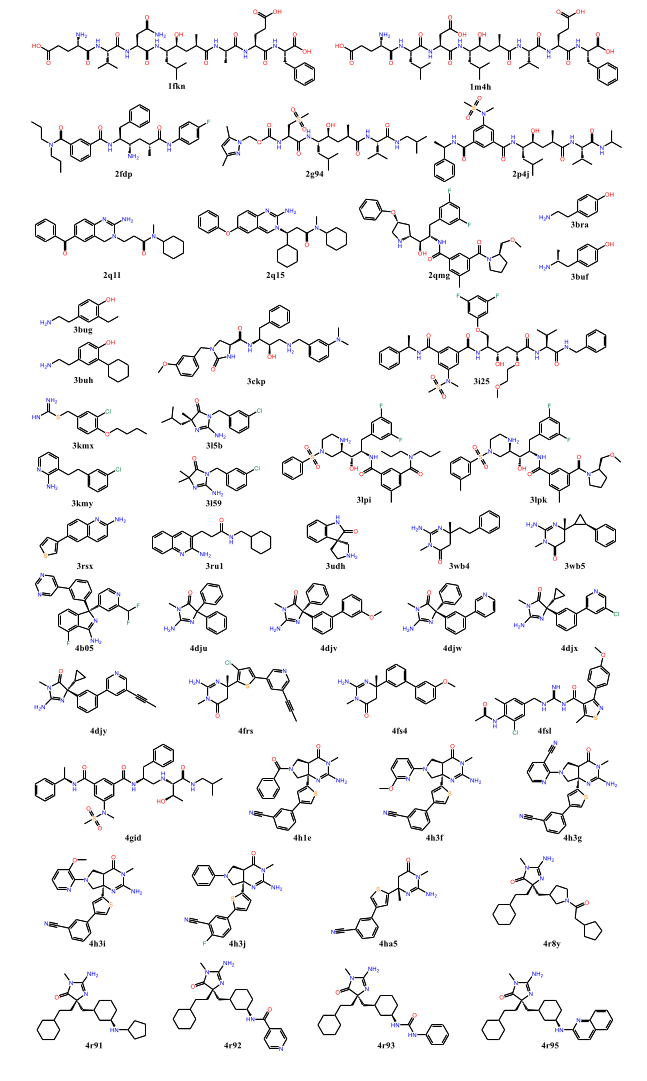
\includegraphics[width=0.8\textwidth]{chapters/Applications/images/structures_mmpbsa.png}}
	\captionof{figure}{Structure 2D des ligands de chaque complexe étudié}
    \label{fig:structures_MMPBSA}
\end{center}







\subsection{Résultats}

La figure \ref{fig:MMPBSA_MMMDFT_complete} compare les énergies libres de solvatation calculées (a) par MM-PBSA, (b) par MM-MDFT avec la correction de pression PC, (c) par MM-MDFT avec la correction de pression PC et (d) par MM-MDFT avec le bridge gros grain, aux valeurs expérimentales pour chacun des 46 complexes protéine-ligands étudiés. Pour chaque jeux de données, nous avons ensuite calculé le coefficient de corrélation $\mathrm{R}^2$ (voir tableau \ref{tab:MMPBSA_correlation}). 


\begin{figure}[H]
    \begin{subfigure}[b]{0.50\textwidth}
        \centering
        \caption{MM-PBSA}
        \resizebox{\linewidth}{!}{
          \begin{tikzpicture}
            \begin{axis}[
                    xlabel= $\Delta \mathrm{G_{liaison}\ exp}\ (\mathrm{kCal.mol}^{-1}$),
                    ylabel= $\Delta \mathrm{G_{liaison}\ calc}\ (\mathrm{kCal.mol}^{-1}$),
                    legend style = {draw = none},
                    xmin = -16, xmax = -2, ymin = -200, ymax = 20,
                    legend entries={$\mathrm{R}^2$=0.66},
                 legend pos=south east]
                 \addlegendimage{only marks,white};
              
              \addplot[only marks,mark=*, black, very thick] table[x index=0, y index=1]{chapters/Applications/datas/MMPBSA/results.csv};
            \end{axis}
          \end{tikzpicture}
          }
     \end{subfigure}%
     \begin{subfigure}[b]{0.50\textwidth}
        \centering
        \caption{$\mathrm{m}_\mathrm{max}$ 1 PC}
        \resizebox{\linewidth}{!}{
          \begin{tikzpicture}
            \begin{axis}[
                    xlabel= $\Delta \mathrm{G_{liaison}\ exp}\ (\mathrm{kCal.mol}^{-1}$),
                    ylabel= $\Delta \mathrm{G_{liaison}\ calc}\ (\mathrm{kCal.mol}^{-1}$),
                    legend style = {draw = none},
                    xmin = -16, xmax = -2, ymin = -200, ymax = 20,
              legend entries={$\mathrm{R}^2$=0.61},
                 legend pos=south east]
                 \addlegendimage{only marks,white};
              \addplot[only marks,mark=*, black, very thick] table[x index=0, y index=2]{chapters/Applications/datas/MMPBSA/results.csv};
            \end{axis}
          \end{tikzpicture}
          }
     \end{subfigure}
     \begin{subfigure}[b]{0.50\textwidth}
        \centering
        \caption{$\mathrm{m}_\mathrm{max}$ 1 PC+}
        \resizebox{\linewidth}{!}{
          \begin{tikzpicture}
            \begin{axis}[
                    xlabel= $\Delta \mathrm{G_{liaison}\ exp}\ (\mathrm{kCal.mol}^{-1}$),
                    ylabel= $\Delta \mathrm{G_{liaison}\ calc}\ (\mathrm{kCal.mol}^{-1}$),
                    legend style = {draw = none},
                    xmin = -16, xmax = -2, ymin = -200, ymax = 20,
              legend entries={$\mathrm{R}^2$=0.62},
                 legend pos=south east]
                 \addlegendimage{only marks,white};
              \addplot[only marks,mark=*, black, very thick] table[x index=0, y index=3]{chapters/Applications/datas/MMPBSA/results.csv};
            \end{axis}
          \end{tikzpicture}
          }
     \end{subfigure}%
     \begin{subfigure}[b]{0.50\textwidth}
        \centering
        \caption{$\mathrm{m}_\mathrm{max}$ 1 + bridge}
        \resizebox{\linewidth}{!}{
          \begin{tikzpicture}
            \begin{axis}[
                    xlabel= $\Delta \mathrm{G_{liaison}\ exp}\ (\mathrm{kCal.mol}^{-1}$),
                    ylabel= $\Delta \mathrm{G_{liaison}\ calc}\ (\mathrm{kCal.mol}^{-1}$),
                    legend style = {draw = none},
                    xmin = -16, xmax = -2, ymin = -200, ymax = 20,
              legend entries={$\mathrm{R}^2$=0.69},
                 legend pos=south east]
                 \addlegendimage{only marks,white};
              \addplot[only marks,mark=*, black, very thick] table[x index=0, y index=4]{chapters/Applications/datas/MMPBSA/results.csv};
            \end{axis}
          \end{tikzpicture}
          }
     \end{subfigure}
    \caption{Énergie libre de liaison calculée par MM-PBSA et par MM-MDFT pour différents paramètres de la fonctionnelle comparée à l'énergie libre de liaison expérimentale pour chacun des complexes étudiés.}
    \label{fig:MMPBSA_MMMDFT_complete}
\end{figure}




Les résultats obtenus avec MM-MDFT sans bridge, avec la correction de pression PC ou PC+ sont légèrement moins bons ($\mathrm{R}^2$=0.61 et $\mathrm{R}^2$=0.62) que ceux obtenus avec MM-PBSA ($\mathrm{R}^2$=0.66). Au contraire, les résultats obtenus avec $\mathrm{m}_\mathrm{max}=1$ et le bridge gros grain, sont quant à eux légèrement plus corrélés que notre référence MM-PBSA aux valeurs expérimentales. En plus de cette amélioration de la prédiction des valeurs d'énergie libre de liaison, dans le même temps, MM-MDFT nous propose les structures de solvatation de la protéine, du ligand ainsi que du complexe.





\begin{table}[H]
  \begin{center}
    \begin{tabular}{ c c }
      \hline & \\[-1em]\hline
       fonctionnelle  & R²  \\
      \hline
       MM-PBSA  & 0.66 \\
  %    \hline
       $\mathrm{m}_\mathrm{max}$ 1 PC  & 0.61  \\
  %    \hline
       $\mathrm{m}_\mathrm{max}$ 1 PC+  & 0.62  \\
  %    \hline
       $\mathrm{m}_\mathrm{max}$ 1 + bridge  & 0.69  \\
  %    \hline
%      e & $\mathrm{m}_\mathrm{max}$ 3 PC  & 0.28  \\
  %    \hline
%      f & $\mathrm{m}_\mathrm{max}$ 3 PC+  & 0.27  \\
  %    \hline
%      g & $\mathrm{m}_\mathrm{max}$ 3 + bridge  & 0.55  \\
  %    \hline
%      h & $\mathrm{m}_\mathrm{max}$ 5 + bridge  & 0.58  \\
      \hline & \\[-1em]\hline%
    \end{tabular}
  \end{center}
  \caption{Coefficient de corrélation entre les valeurs d'énergie libre de liaisons calculées et les valeurs expérimentales.}
  \label{tab:MMPBSA_correlation}  
\end{table}


Les systèmes étudiés sont composés de nombreux halogènes et ne sont pas représentatifs de l'espace chimique. Afin de nous assurer que MDFT n'était pas biaisé par rapport à certains composés, nous avons dans un premier temps coloré les points en fonction des halogènes qu'il contenaient ( voir figure \ref{fig:MMPBSA_MMMDFT_complete_by_halogene} ). Dans un second temps nous avons coloré les composés contenant au moins un atome de Souffre. Dans les deux cas, les différentes catégories sont uniformément réparties dans le nuage de point. Le souffre ainsi que les différents halogènes présents sont donc correctement modélisés.


\begin{figure}[H]
    \begin{subfigure}[b]{0.50\textwidth}
        \centering
        \caption{MM-PBSA}
        \resizebox{\linewidth}{!}{
          \begin{tikzpicture}
            \begin{axis}[
                    xlabel= $\Delta \mathrm{G_{liaison}\ exp}\ (\mathrm{kCal.mol}^{-1}$),
                    ylabel= $\Delta \mathrm{G_{liaison}\ calc}\ (\mathrm{kCal.mol}^{-1}$),
                    legend pos=south east,
                    xmin = -16, xmax = -2, ymin = -200, ymax = 20,
              ]
              \addplot[
        scatter,only marks,scatter src=explicit symbolic,
        scatter/classes={
            Fluor={red},
            Chlore={blue},
            None={black}
        }
    ] table[x index=0, y index=1, meta index=10]{chapters/Applications/datas/MMPBSA/results.csv};
            \legend{Cl, F, Aucun,};
            \end{axis}
          \end{tikzpicture}
          }
     \end{subfigure}
     \begin{subfigure}[b]{0.50\textwidth}
        \centering
        \caption{$\mathrm{m}_\mathrm{max}$ 1 PC}
        \resizebox{\linewidth}{!}{
          \begin{tikzpicture}
            \begin{axis}[
                    xlabel= $\Delta \mathrm{G_{liaison}\ exp}\ (\mathrm{kCal.mol}^{-1}$),
                    ylabel= $\Delta \mathrm{G_{liaison}\ calc}\ (\mathrm{kCal.mol}^{-1}$),
                    legend pos=south east,
                    xmin = -16, xmax = -2, ymin = -200, ymax = 20,
              ]
              \addplot[
        scatter,only marks,scatter src=explicit symbolic,
        scatter/classes={
            Fluor={red},
            Chlore={blue},
            None={black}
        }
    ] table[x index=0, y index=2, meta index=10]{chapters/Applications/datas/MMPBSA/results.csv};
            \legend{Cl, F, Aucun,};
            \end{axis}
          \end{tikzpicture}
          }
     \end{subfigure}
     \begin{subfigure}[b]{0.50\textwidth}
        \centering
        \caption{$\mathrm{m}_\mathrm{max}$ 1 PC+}
        \resizebox{\linewidth}{!}{
          \begin{tikzpicture}
            \begin{axis}[
                    xlabel= $\Delta \mathrm{G_{liaison}\ exp}\ (\mathrm{kCal.mol}^{-1}$),
                    ylabel= $\Delta \mathrm{G_{liaison}\ calc}\ (\mathrm{kCal.mol}^{-1}$),
                    legend pos=south east,
                    xmin = -16, xmax = -2, ymin = -200, ymax = 20,
              ]
              \addplot[
        scatter,only marks,scatter src=explicit symbolic,
        scatter/classes={
            Fluor={red},
            Chlore={blue},
            None={black}
        }
    ] table[x index=0, y index=3, meta index=10]{chapters/Applications/datas/MMPBSA/results.csv};
            \legend{Cl, F, Aucun,};
            \end{axis}
          \end{tikzpicture}
          }
     \end{subfigure}
     \begin{subfigure}[b]{0.50\textwidth}
        \centering
        \caption{$\mathrm{m}_\mathrm{max}$ 1 + bridge}
        \resizebox{\linewidth}{!}{
          \begin{tikzpicture}
            \begin{axis}[
                    xlabel= $\Delta \mathrm{G_{liaison}\ exp}\ (\mathrm{kCal.mol}^{-1}$),
                    ylabel= $\Delta \mathrm{G_{liaison}\ calc}\ (\mathrm{kCal.mol}^{-1}$),
                    legend pos=south east,
                    xmin = -16, xmax = -2, ymin = -200, ymax = 20,
              ]
              \addplot[
        scatter,only marks,scatter src=explicit symbolic,
        scatter/classes={
            Fluor={red},
            Chlore={blue},
            None={black}
        }
    ] table[x index=0, y index=4, meta index=10]{chapters/Applications/datas/MMPBSA/results.csv};
            \legend{Cl, F, Aucun,};
            \end{axis}
          \end{tikzpicture}
          }
     \end{subfigure}
    \caption{Énergie libre de liaison calculée par MM-PBSA et par MM-MDFT pour différents paramètres de la fonctionnelle comparée à l'énergie libre de liaison expérimentale pour chacun des complexes étudiés. Les complexes dont le ligand comporte au moins un Chlore sont représentés en rouge. Ceux qui comportent au moins un Fluor sont en bleu et ceux ne comportant pas d'halogène sont en noir. }
    \label{fig:MMPBSA_MMMDFT_complete_by_halogene}
\end{figure}








\begin{figure}[H]
    \begin{subfigure}[b]{0.50\textwidth}
        \centering
        \caption{MM-PBSA}
        \resizebox{\linewidth}{!}{
          \begin{tikzpicture}
            \begin{axis}[
                    xlabel= $\Delta \mathrm{G_{liaison}\ exp}\ (\mathrm{kCal.mol}^{-1}$),
                    ylabel= $\Delta \mathrm{G_{liaison}\ calc}\ (\mathrm{kCal.mol}^{-1}$),
                    legend pos=south east,
                    xmin = -16, xmax = -2, ymin = -200, ymax = 20,
              ]
              \addplot[
        scatter,only marks,scatter src=explicit symbolic,
        scatter/classes={
            Sulfure={red},
            None={black}
        }
    ] table[x index=0, y index=1, meta index=11]{chapters/Applications/datas/MMPBSA/results.csv};
            \legend{Avec S, Sans S};
            \end{axis}
          \end{tikzpicture}
          }
     \end{subfigure}
     \begin{subfigure}[b]{0.50\textwidth}
        \centering
        \caption{$\mathrm{m}_\mathrm{max}$ 1 PC}
        \resizebox{\linewidth}{!}{
          \begin{tikzpicture}
            \begin{axis}[
                    xlabel= $\Delta \mathrm{G_{liaison}\ exp}\ (\mathrm{kCal.mol}^{-1}$),
                    ylabel= $\Delta \mathrm{G_{liaison}\ calc}\ (\mathrm{kCal.mol}^{-1}$),
                    legend pos=south east,
                    xmin = -16, xmax = -2, ymin = -200, ymax = 20,
              ]
              \addplot[
        scatter,only marks,scatter src=explicit symbolic,
        scatter/classes={
            Sulfure={red},
            None={black}
        }
    ] table[x index=0, y index=2, meta index=11]{chapters/Applications/datas/MMPBSA/results.csv};
            \legend{Avec S, Sans S};
            \end{axis}
          \end{tikzpicture}
          }
     \end{subfigure}
     \begin{subfigure}[b]{0.50\textwidth}
        \centering
        \caption{$\mathrm{m}_\mathrm{max}$ 1 PC+}
        \resizebox{\linewidth}{!}{
          \begin{tikzpicture}
            \begin{axis}[
                    xlabel= $\Delta \mathrm{G_{liaison}\ exp}\ (\mathrm{kCal.mol}^{-1}$),
                    ylabel= $\Delta \mathrm{G_{liaison}\ calc}\ (\mathrm{kCal.mol}^{-1}$),
                    legend pos=south east,
                    xmin = -16, xmax = -2, ymin = -200, ymax = 20,
              ]
              \addplot[
        scatter,only marks,scatter src=explicit symbolic,
        scatter/classes={
            Sulfure={red},
            None={black}
        }
    ] table[x index=0, y index=3, meta index=11]{chapters/Applications/datas/MMPBSA/results.csv};
            \legend{Avec S, Sans S};
            \end{axis}
          \end{tikzpicture}
          }
     \end{subfigure}
     \begin{subfigure}[b]{0.50\textwidth}
        \centering
        \caption{$\mathrm{m}_\mathrm{max}$ 1 + bridge}
        \resizebox{\linewidth}{!}{
          \begin{tikzpicture}
            \begin{axis}[
                    xlabel= $\Delta \mathrm{G_{liaison}\ exp}\ (\mathrm{kCal.mol}^{-1}$),
                    ylabel= $\Delta \mathrm{G_{liaison}\ calc}\ (\mathrm{kCal.mol}^{-1}$),
                    legend pos=south east,
                    xmin = -16, xmax = -2, ymin = -200, ymax = 20,
              ]
              \addplot[
        scatter,only marks,scatter src=explicit symbolic,
        scatter/classes={
            Sulfure={red},
            None={black}
        }
    ] table[x index=0, y index=4, meta index=11]{chapters/Applications/datas/MMPBSA/results.csv};
            \legend{Avec S, Sans S};
            \end{axis}
          \end{tikzpicture}
          }
     \end{subfigure}
    \caption{Énergie libre de liaison calculée par MM-PBSA et par MM-MDFT pour différents paramètres de la fonctionnelle comparée à l'énergie libre de liaison expérimentale pour chacun des complexes étudiés. En rouge les complexes dont le ligand comporte un Souffre, en noir ceux n'en comportant pas.}
    \label{fig:MMPBSA_MMMDFT_complete_by_souffre}
\end{figure}







%Les meilleurs résultats obtenus avec MM-MDFT, le sont pour $\mathrm{m}_\mathrm{max}$ 1 avec le bridge gros grain. Dans cette configuration MM-MDFT à une corrélation par rapport aux valeurs expérimentales $\mathrm{R}^2$=0,69 pour 0,66 avec MM-PBSA (voir figure \ref{fig:MMPBSA_MMMDFT_complete}. Tous les autres paramètres de la fonctionnelle donnent une corrélation plus basse que MM-PBSA. Les résultats obtenus pour un $\mathrm{m}_\mathrm{max}$ 1 sans bridge, ainsi que pour $\mathrm{m}_\mathrm{max}$ 3 et 5 avec le bridge gros grain restent proches de notre référence avec un $\mathrm{R}^2$ compris entre 0,58 et 0,62. Les résultats obtenus avec $\mathrm{m}_\mathrm{max}$ 3 sans bridge sont par contre. Nous rappelons au lecteur, que MM-MDFT fourni, en plus des énergies libre de liaison, les structures de solvatation des complexes et des composés initiaux.


%Les résultats obtenus pour $\mathrm{m}_\mathrm{max}$ 3 sans bridges sont plus surprenants, ils sont complètement décorrélés des valeurs expérimentales $\mathrm{R}^2$ inférieur à 0,3. Cela peut être expliqué par le caractère préliminaire et très simplifié de cette application. 



En conclusion, nous avons montré dans ce chapitre que les calculs MDFT avec notre nouveau bridge et $\mathrm{m}_\mathrm{max}$=1 améliore les résultats tout en apportant le détail des structures de solvant autour de la protéine, du ligand et du complexe, dans des temps de calculs similaires à MM-PBSA. Nous rappelons également au lecteur, que les résultats MM-PBSA ont été optimisés pour cette protéine, ce qui n'est pas le cas des calculs MDFT. Nous avons ici utilisé nos paramètres par défaut soit l'eau SPC/E avec une force ionique nulle. Cheron et Al ont montré que ces paramètres sont sous-optimums, et ont eux utilisé de l'eau TIP3P et une force ionique 3M.




\subsection{Perspectives}
Dans cette étude préliminaire, nous n'avons considéré qu'une seule conformation par complexe, la conformation après minimisation de la structure cristallographique. A cause des conditions expérimentales nécessaires à la résolution de structures de systèmes biologiques en 3 dimensions, les conformations obtenues sont plus ou mois éloignées de celles présentes en solution dans les conditions standards. Afin de minimiser ces différences, il est possible de calculer une trajectoire de dynamique moléculaire ou Monte Carlo du complexe dans le vide et d'en extraire différentes conformations à intervalle régulier. 
L'énergie libre de solvatation du système correspond, dans ce cas, à la moyenne des énergies libre de solvatation calculées pour chaque conformation. Pour MM-PBSA, l'utilisation de cette méthode, appelée communément "l'approximation de trajectoire unique", permet d'améliorer la corrélation de MM-PBSA à $\mathrm{R}^2$=0.71. Au moment de la rédaction de ce rapport, des calculs similaires était en cours pour MM-MDFT.


 \vspace{8\baselineskip}


\boitemagique{A Retenir}{
Dans ce chapitre, nous avons montré qu'il est possible avec MDFT (i) d'étudier avec précision des systèmes biologiques, (ii) de retrouver les molécules d'eau expérimentales et les poches à l'intérieur de protéines et (iii) d'améliorer la prédiction d'énergie libre de liaison en solution tout en fournissant la structure de solvatation.
}


